\documentclass[preprint,12pt]{elsarticle}

\usepackage{bm}% bold math
\usepackage{amsmath}
\usepackage{color}  
\usepackage{amssymb}
\usepackage{placeins}
\usepackage{caption}
\usepackage{subcaption}
\usepackage[margin=2.5cm]{geometry}
\usepackage{graphicx} % Required for inserting images
\usepackage{booktabs}
\usepackage{comment}
\usepackage{tabularx}
\usepackage{hyperref}
\usepackage{cleveref}

\journal{Journal of Nuclear Materials}

\title{Bulk and Surface Diffusion of Lanthanides (Ce and  Nd) and Actinides (U and Pu) in Body-Centered Cubic Fe}

\author[inst1]{Shehab Shousha}
\affiliation[inst1]{organization={North Carolina State University},%Department and Organization
            city={Raleigh},
            state={NC},
            postcode={27695}, 
            country={United States}}

\author[inst1,inst2]{Benjamin Beeler}
\affiliation[inst2]{organization={Idaho National Laboratory},%Department and Organization 
            city={Idaho Falls},
            state={ID},
            postcode={83415}, 
            country={United States}}


\author[inst2,inst3]{Larry K. Aagesen}
\affiliation[inst3]{organization={Department of Nuclear Engineering and Radiological Sciences, University of Michigan},%Department and Organization 
            city={Ann Arbor},
            state={MI},
            postcode={48109}, 
            country={United States}}

\author[inst2]{Geoffrey L. Beausoleil II}
\author[inst4]{Maria A. Okuniewski}
\affiliation[inst4]{organization={Purdue University},%Department and Organization 
            city={West Lafayette},
            state={IN},
            postcode={47907}, 
            country={United States}}


\date{\today}

\begin{document}

\begin{abstract}
Fuel-cladding chemical interaction (FCCI) is a major degradation mechanism in sodium-cooled fast reactors, driven by the diffusion of lanthanide fission products and actinide fuel constituents into Fe-based cladding.  To elucidate this phenomenon, we used density functional theory and self-consistent mean field theory to calculate the vacancy-mediated diffusivities of Ce, Nd, U, and Pu in body-centered cubic Fe. Our findings reveal that all solutes exhibit accelerated diffusion relative to Fe, primarily due to strong vacancy drag effects. Additionally, we investigated surface diffusion via the vacancy mechanism on the Fe (110) surface, which serves as a proxy for grain boundary (GB) diffusion. The results indicate that the surface diffusion is significantly faster than bulk diffusion, with activation energies reduced by 0.7–0.9 eV. While vacancy-mediated transport is likely for oversized solutes, GB self-diffusion mechanisms remain uncertain. These insights provide critical inputs for the development of multiscale FCCI models, advancing our understanding of material degradation in next-generation nuclear reactors. 
\end{abstract}

\maketitle

\section{Introduction}

\noindent Fuel-cladding chemical interaction (FCCI) is a critical concern in sodium-cooled fast reactors \cite{hofman_metallic_1997, pahl_experimental_1990, thomas_nano-mechanical_2021} and is widely recognized as one of the leading causes of fuel-pin failures \cite{matthews_fuel-cladding_2017}. FCCI involves the interdiffusion between fuel and cladding materials, which weakens the cladding and leads to the formation of brittle and low-melting-point phases. Notably, the diffusion of lanthanide fission products such as Nd, Ce, and La into HT9 cladding results in the formation of intermetallic compounds such as $(Fe, Cr)_{17}(Nd, Ce, La)_{2}$ \cite{keiser_fuel-cladding_2006, harp_scanning_2017}. Additionally, interdiffusion at the fuel-cladding interface—particularly the diffusion of Fe toward the fuel side—leads to the formation of (U,Pu)/Fe eutectics, which can dissolve the cladding at elevated temperatures and thereby accelerate the ingress of fuel constituents (U and Pu) into Fe-based alloys \cite{matthews_fuel-cladding_2017, keiser2009development, cohen1993fuel}.

A fundamental understanding of the diffusion of lanthanide and actinide species in Fe-based cladding is essential for developing accurate multiscale models of the FCCI in metallic fuels \cite{aagesen_jr_physics-based_2022, aagesen_mechanistic_2023}. One approach to evaluate the diffusivity of these species in Fe is through diffusion couple measurements. Several studies have reported diffusion couple experiments on lanthanide/Fe alloys \cite{INAGAKI2013574, JERRED2020152387, helmreich_diffusion_2014}, but only one has provided interdiffusion coefficients for the Nd/HT9 system \cite{helmreich_diffusion_2014}. Diffusion couple data are also available for the U/Fe system \cite{huang2012interdiffusion, chen2015intermetallic}, and these measurements are physically relevant since, after fuel swelling, the fuel-cladding gap can close under irradiation, creating direct U-Fe contact. In contrast, the interdiffusion coefficients obtained from lanthanide/Fe diffusion couples may only provide a qualitative indication of in-reactor behavior, as lanthanides are gradually generated as fission products rather than introduced as preexisting alloys, as they are in diffusion couples. Consequently, the transport of lanthanides into Fe-based cladding is more appropriately modeled as dilute solute diffusion. This dilute diffusion behavior is also essential when considering mitigation strategies such as Zr liners or Cr coatings \cite{ryu_performance_2009, kim_performance_2009, jee_improvement_2013, OH2024113102}, where lanthanide and actinide penetration into the cladding occurs at low concentrations rather than through bulk interdiffusion.


\textit{Ab initio} calculations have been proven effective in studying the transport of solute atoms at dilute concentrations. Extensive research on solute diffusion in body-centered cubic (BCC) Fe has been conducted using density functional theory (DFT) \cite{messina_exact_2014, murali_bcc_fe_2015, versteylen_first-principles_2017}. For vacancy-mediated diffusion, solute diffusivities can be obtained by incorporating DFT-derived energetics into analytical models such as the nine-frequency model \cite{leclaire1970}. Versteylen \textit{et al.} \cite{versteylen_first-principles_2017} applied this approach to calculate solute diffusivities for 27 different species in BCC Fe. Although the nine-frequency model provides a useful framework for calculating solute diffusivities, it underestimates vacancy drag effects due to its approximate nature \cite{messina_exact_2014}. To address this limitation, an exact method for calculating solute transport coefficients was developed within the framework of self-consistent mean field (SCMF) theory \cite{nastar_self-consistent_2000, nastar_mean_2005}. Messina \textit{et al.} \cite{messina_exact_2014} applied the SCMF method to predict the exact transport coefficients of solutes in BCC Fe. This method was later generalized by Schuler  \textit{et al.} through the KineCluE code \cite{schuler_kineclue_2020} using a cluster expansion approach \cite{schuler_transport_2016}. This approach enables the accurate prediction of vacancy drag effects by calculating exact transport coefficients for any crystal structure and defect configuration.

For oversized solutes, vacancy-solute pairs form a defect complex where the solute atom occupies an off-lattice site between two half-vacancies \cite{bocquet_migration_2017}. The atomic jumps 
arising from these configurations are not treated in the standard nine-frequency model.
Bocquet \textit{et al.} \cite{bocquet_migration_2017} developed a modified nine-frequency model \cite{leclaire1970} to resolve this for Y in BCC Fe. Building on this, Yang \textit{et al.} \cite{yang_significant_2023} applied DFT alongside Bocquet’s oversized solute atom (OSA) model to determine Nd, Ce, and La diffusion coefficients in both BCC Fe and Cr. Similarly, Lin \textit{et al.} \cite{lin2024first} utilized this approach to calculate the diffusivities of Cs and I in BCC Cr. However, the transport coefficients for oversized solutes in BCC Fe have not been accurately calculated using the SCMF method. Furthermore, to the best of our knowledge, no DFT studies have investigated the diffusion of U and Pu in BCC Fe prior to this work.

Experiments have shown the infiltration of lanthanide fission products along HT9 grain boundaries (GBs) \cite{wang2022small, wang2024transmission}, suggesting that GBs play a crucial role in FCCI. However, the diffusivities of lanthanides and actinides along the GBs and surfaces of Fe have not been investigated according to our review of the literature. Understanding these is essential for developing accurate engineering-scale models of the FCCI.

In this work, DFT and the SCMF method are employed, as implemented in the KineCluE code \cite{schuler_kineclue_2020}, to calculate the exact transport coefficients of Ce, Nd, U, and Pu in BCC Fe via the vacancy-mediated mechanism. This mechanism is well accepted for describing the diffusion of the OSA in BCC lattices \cite{ bocquet_migration_2017,yang_significant_2023}. Using these transport coefficients, we evaluate solute diffusivities, vacancy drag effects, and segregation tendencies in bulk Fe. This methodology builds on our prior work investigating lanthanide diffusion in hexagonally close-packed Zr \cite{shousha2024first} and BCC Cr and V \cite{shousha_cr}. 

In addition to bulk behavior, we also examine the vacancy-mediated diffusion of Ce, Nd, U, and Pu on the Fe (110) surface using DFT and the SCMF method. Direct modeling of grain boundary diffusion using DFT is computationally intensive due to the large supercells, complex atomic arrangements, and the need for extensive configurational sampling. To overcome these challenges, we use diffusion on a low-index surface as a proxy for diffusion along grain boundaries. These boundaries often exhibit undercoordinated, disordered, or surface-like atomic environments, making surface diffusion a reasonable analog for capturing qualitative trends in GB transport behavior. This similarity between surface and GB diffusivities was also emphasized by Taylor \textit{et al.} \cite{taylor2024directly} in their experimental study to measure surface self-diffusivities in Fe.
The results of this study provide first-principles-based diffusion data for Ce, Nd, U, and Pu in Fe, supporting the development of multiscale models for the FCCI.

%Lanthanide segregation to grain boundaries \cite{cao_segregation_2019}


\FloatBarrier
\section{Methodology}
\FloatBarrier
\subsection{Evaluation of Transport Coefficients}

\noindent The Onsager transport coefficients, $L_{ij}$, relate the flux $J_i$ of species $i$ to the chemical potential gradient $\mu_j$ of species $j$ according to the following relationship \cite{allnatt_atomic_2003}:

\begin{equation}
   J_i = -\sum_j{L_{ij} \frac{\nabla\mu_j}{k_B T}} ,
\label{eq_onsager}
\end{equation}
where $k_B$ is Boltzmann's constant. In this work, the diffusing species considered are vacancies (\textit{V}) and solutes (\textit{B}). Accordingly, the $L_{ij}$ coefficients can be expressed in matrix form and \Cref{eq_onsager} can be rewritten as:

\begin{equation}
\label{matrix_form_onsager}
    \begin{bmatrix}
        J_V \\
        J_B 
    \end{bmatrix}=\frac{-1}{k_B T}
    \begin{bmatrix}
    L_{VV} & L_{VB} \\
    L_{VB} & L_{BB}
    \end{bmatrix}
        \begin{bmatrix}
        \nabla\mu_V \\
        \nabla\mu_B
    \end{bmatrix}.
\end{equation}

\noindent The $L_{ij}$ coefficients are calculated using the SCMF method \cite{nastar_self-consistent_2000, nastar_mean_2005} and the cluster expansion approach as implemented in KineCluE \cite{schuler_kineclue_2020}. This is done by calculating the transport coefficients for clusters containing only vacancies, $L_{ij}^{(V)}$, and clusters containing a vacancy-solute pair, $L_{ij}^{(VB)}$. Then, the weighted contributions from both types of clusters are combined as follows:

\begin{equation}
\label{eq_onsager_matrix}
\begin{bmatrix}
L_{VV} & L_{VB} \\
L_{VB} & L_{BB}
\end{bmatrix}
=
C \Biggl(
f_V 
\begin{bmatrix}
{L_{VV}}^{(V)} & 0 \\
0 & 0 
\end{bmatrix}
+ f_{VB}
\begin{bmatrix}
{L_{VV}}^{(VB)} & {L_{VB}}^{(VB)} \\
{L_{VB}}^{(VB)} & {L_{BB}}^{(VB)}
\end{bmatrix}
\Biggr),
\end{equation}
where $C$ is the total concentration of sites occupied by vacancies or vacancy-solute pairs, and $f_V$ and $f_{VB}$ are the fractions of single-vacancy and vacancy-solute clusters, respectively. The quantities $C$, $f_V$, and $f_{VB}$ are calculated using the partition functions evaluated by KineCluE \cite{schuler_kineclue_2020}, as explained in our previous works \cite{shousha2024first, shousha_vacancy-mediated_2024} and in the work of Messina \textit{et al.} \cite{messina_solute_2020}.

The solute diffusivities in the dilute limit, $D_B$, are calculated using the transport coefficient, $L_{BB}$, as follows:
\begin{equation}
\label{eq_solute_diffusivity}
    D_B = \frac{L_{BB}}{C_B},
\end{equation}
where $C_B$ is the concentration of the solute (\textit{B}).  The diffusivity \( D_B \) is effectively independent of the solute concentration \( C_B \) within the dilute limit, defined as $C_B < [B]_{max}$. According to our model, this dilute limit corresponds to a maximum solute concentration of $[B]_{max} = \frac{1}{540} = 0.185\%$. This value is determined by the cluster size ($r_{kin} = 4 a_0$) employed in KineCluE \cite{schuler_kineclue_2020}, where \( a_0 \) is the lattice parameter of BCC Fe. Increasing the kinetic range ($r_{kin}$) allows for the inclusion of more long-range kinetic correlations but reduces the allowable dilute concentration range, and vice versa. Nevertheless, a range of \( 4a_0 \) yields well-converged transport coefficients. Similarly, for two-dimensional surface diffusion, a cluster size of ($r_{kin} = 5 a_0$) results in converged results and is used in calculating surface diffusion coefficients. This value corresponds to a maximum solute concentration of $[B]_{max} = \frac{1}{86} = 1.163\%$ on the surface. For a detailed discussion, see references \cite{shousha2024first, shousha_vacancy-mediated_2024, messina_solute_2020}.
The self-diffusion coefficient of Fe is determined by introducing a solute (\textit{B}) that has the same energetics as the host atoms, effectively serving as a tracer atom.

In addition to evaluating diffusivities, the transport coefficients are utilized to estimate the solute segregation tendencies due to the flux coupling with vacancies. This is performed by using the off-diagonal transport coefficients to evaluate the vacancy drag ratios $G_V$ and the partial diffusion coefficient ratios $D_{pd}$ as follows \cite{messina_exact_2014, messina_solute_2020}:
\begin{equation}
\label{eq:drag}
    G_V = \frac{L_{VB}^{(VB)}}{L_{BB}^{(VB)}}
\end{equation}

\begin{equation}
\label{eq:pdc}
D_{pd} = \frac{(1-C_B)}{C_B} \frac{L_{VB}}{L_{AV}}.
\end{equation}

\noindent The vacancy drag ratio in \Cref{eq:drag} indicates whether a solute diffuses in the same direction of the vacancy flux  ($G_V > 0$, due to vacancy drag) or in the opposite direction ($G_V < 0$, known as the inverse Kirkendall effect, IKE \citep{marwick_segregation_1978}). The value of \( D_{pd} \) in \Cref{eq:pdc} characterizes solute behavior near vacancy sinks (e.g., grain boundaries), indicating tendencies for enrichment or depletion \citep{messina_exact_2014}. When \( D_{pd} < 0 \), solutes follow the vacancy flux (\( G_V > 0 \)), leading to enrichment due to vacancy drag. For \( D_{pd} > 1 \), solutes diffuse faster than host atoms and move opposite to the vacancy flux (\( G_V < 0 \)), resulting in depletion. In the intermediate range \( 0 < D_{pd} < 1 \), both solutes and host atoms move opposite to the vacancy flux, but slower solute diffusion leads to enrichment at sinks \cite{messina_exact_2014}.

\FloatBarrier
\subsection{Ab Initio Methodology}

\noindent DFT calculations were performed using the projector-augmented wave (PAW) method as implemented in the Vienna Ab initio Simulation Package (VASP) \cite{kresse_ab_1993, kresse_efficient_1996}. The exchange-correlation interactions were treated using the Perdew--Burke--Ernzerhof generalized gradient approximation (GGA) \cite{perdew_generalized_1996}. A plane-wave cutoff energy of 450 eV and a first-order Methfessel--Paxton smearing with a width of 0.2 eV were employed \cite{methfessel_high-precision_1989} in all calculations. Spin-polarized calculations with collinear magnetic moments were used to model the ferromagnetic $\alpha$-Fe phase, resulting in a relaxed BCC Fe structure with a magnetic moment of 2.18 $\mu$B per atom. The pseudopotentials utilized are those recommended from VASP, with a valence of 8 electrons for Fe, 12 electrons for Ce, 11 electrons for Nd, 14 electrons for U, and 16 electrons for Pu. 

For bulk diffusion calculations, supercells of 128 atoms were generated by duplicating the conventional BCC unit cell $4\times4\times4$ times.  The Brillouin zone was sampled using a $4\times4\times4$ $\Gamma$-centered k-point mesh without using the symmetry operations in VASP, which results in 64 k-points in the irreducible Brillouin zone. 
For surface diffusion calculations, the close-packed (110) surface is chosen. Its high atomic packing density minimizes surface energy, making it the predominant surface \cite{tran2016surface}. To model this surface, a slab of 216 atoms is constructed with 6 atomic layers with 36 atoms per layer and a vacuum separation of $\sim$13 {\AA} along the [110] direction, utilizing initial input from the Grain Boundary Database \cite{tran2016surface, zheng_grain_2020}. The Brillouin zone was sampled using a $4\times4\times2$ $\Gamma$-centered k-point mesh. During geometry relaxation, the convergence criteria for total energies and forces were set to $10^{-6}$ eV and 0.01 eV/{\AA}, respectively, unless noted otherwise. All geometry relaxations for defect-containing supercells were conducted under a fixed-volume constraint.

The formation, binding, and migration energies of vacancies and solute-vacancy pairs are calculated using DFT energetics. The vacancy formation energy, $E_{form}^{vac}$, is evaluated as follows:
\begin{equation}
\label{eq_Ef_vac}
   E_{form}^{vac} = E^{vac}_{defect}[(N-1)Fe] - \frac{N-1}{N} E_{perfect}[(N) Fe] .
\end{equation}
The terms $E_{perfect}[(N) Fe]$ and $E^{vac}_{defect}[(N-1)Fe]$ are the DFT energies of the perfect and defect-containing supercells, respectively. The number of atoms in the perfect supercell, $N$, is 128 and 216 in the bulk and surface calculations, respectively. Similarly, the substitutional formation energy of a solute $B$, $E_{form}^{sub,B}$, and the formation energy of a solute-vacancy complex, $E_{form}^{sub-vac,B}$, are evaluated as follows:
\begin{equation}
\label{eq_Ef_sub}
    E_{form}^{sub,B} = E_{defect}^{sub}[(N-1)Fe + B] - \frac{N-1}{N}E_{perfect}[(N) Fe] - E_{B},
\end{equation}

\begin{equation}
\label{eq_Ef_vac_sub}
    E_{form}^{sub-vac,B} = E_{defect}^{sub-vac}[(N-2)Fe + B] - \frac{N-2}{N}E_{perfect}[(N) Fe] - E_{B},
\end{equation}
where $E_{defect}^{sub}[(N-1)Fe + B]$ and $E_{defect}^{sub-vac}[(N-2)Fe + B]$ are the DFT energies of supercells containing one substitutional atom and a substitutional-vacancy pair, respectively, of species $B$. The reference energy, $E_{B}$, is the DFT energy per atom for species $B$ in its pure metallic form. These forms are face-centered cubic Ce, double hexagonally closed-packed Nd, orthorhombic U, and monoclinic Pu. The solute-vacancy binding energy, $E_{bind}^{sub-vac,B}$, is given by:
\begin{equation}
\label{eq_Eb}
    E_{bind}^{sub-vac,B} = E_{form}^{vac} + E_{form}^{sub,B} - E_{form}^{sub-vac,B}.
\end{equation}
In this expression, a positive binding energy denotes attraction, and a negative binding energy denotes repulsion. 

The equilibrium concentration of vacancies per atom, $C_V$, at a given temperature, \textit{T}, is calculated according to the following expression:

\begin{equation}
\label{eq:conc_vac}
    C_V = e^{(\frac{-E_{form}^{vac}}{k_B T})} e^{(\frac{S_{form}^{vac}}{k_B}),}
\end{equation}
where $S_{form}^{vac}$ is the vacancy formation entropy. 

The vacancy formation entropy, $S_{form}^{vac}$, is evaluated as follows:
\begin{equation}
    S_{form}^{vac} = k_B ln\left(\frac{\Pi^{3N}_j \nu_j^{perfect}}{\Pi^{3N}_j \nu_j^{def}}\right),
\label{eq_entropy}
\end{equation}
where $\nu_j^{perfect}$ and $\nu_j^{def}$ denote the vibrational frequencies of the selectively dynamic atoms in the perfect and defective supercells, respectively. In principle, $N$ corresponds to the total number of atoms in the defect-free supercell. However, to reduce the computational cost of DFT-based phonon calculations, the harmonic approximation is applied only to atoms within the first- and second-nearest-neighbor (1nn and 2nn) shells of the vacancy site. For surface calculations, this includes $N = 10$ atoms surrounding the vacancy on the (110) surface, which are allowed to vibrate using selective dynamics in VASP (\texttt{IBRION = 5}), while all other atoms remain fixed. As a result, rigid-body translational modes are not present, and all $3N$ vibrational frequencies are used directly in the entropy evaluation. For bulk Fe, the value of $S_{\text{form}}^{\text{vac}}$ is adopted from accurate, full-cell calculations in the literature \cite{messina_systematic_2016}.

To calculate migration barriers, the climbing image nudged elastic band (CI-NEB) method \cite{henkelman_climbing_2000} was employed. A single image was used for all jumps except for those involving the configuration of two half-vacancies. For these jumps, three intermediate images were used, with a less stringent force convergence criterion of 0.05 eV/{\AA} due to challenges achieving convergence below this threshold.


Finally, the attempt frequency from a configuration $i$ to $f$, $\nu^{i\rightarrow f}$, is calculated by an approximate form of Vineyard's harmonic transition state theory \cite{vineyard_frequency_1957} as follows:

\begin{equation}
    \label{eq:attempt_freq}
    \nu^{i\rightarrow f} = \frac{\Pi^{3N_{hop}}_j  \nu^{i}_j}{\Pi^{3N_{hop}-1}_j  \nu^{s,i\rightarrow f}_j},
\end{equation}
where $N_{hop}$ is the number of hopping atoms, and $\nu^{i}$ and $\nu^{s,i\rightarrow f}$ are the vibrational frequencies of the relaxed initial ($i$) state and the saddle point ($s$), respectively. For simplicity, the attempt frequency for the Fe-vacancy jump in pure BCC Fe is adopted from theoretical calculations in the literature \cite{messina_systematic_2016} for bulk diffusion. For surface diffusion, \Cref{eq:attempt_freq} is applied
assuming $N_{hop}=1$, which corresponds to Fe-vacancy and solute-vacancy exchange jumps.


\FloatBarrier
\section{Results}

\subsection{Point Defects in Bulk Fe}

\noindent The bulk properties and the defect energetics in pure BCC Fe are presented in \Cref{tab:bulk_properties}. The calculated lattice parameter, vacancy formation, and migration energies agree well with previous DFT studies \cite{messina_exact_2014, murali_bcc_fe_2015, yang_significant_2023, Li_magnetic_2021, choudhury2011ab} and experiments \cite{kittel2018introduction, schepper_positron1983, tapasa2007computer}. In this study, the vacancy formation entropy ($S_{form}^{vac}$) and the attempt frequency ($\nu$) values are adopted from reference \cite{messina_systematic_2016}. 

\begin{comment}
The calculated phonon-related quantities, $S_{form}^{vac}$ and $\nu$, have lower values than reported by Messina \textit{et al.} \cite{messina_systematic_2016} and Versteylen \textit{et al.} \cite{versteylen_first-principles_2017}. The calculations performed by Messina \textit{et al.} \cite{messina_systematic_2016} are arguably more accurate than our calculations because the vibrational frequencies of all the atoms in the supercell were accounted for. In this study, we only consider the vibrational frequencies of the hopping atom in the case of attempt frequencies and the frequencies of the $2^{nd}$ nearest neighbor shell in the case of $S_{form}^{vac}$. However, it should be noted that errors in $\nu$ and $S_{form}^{vac}$ should not affect the diffusion activation energies and would only perturb the diffusion prefactors by one order of magnitude at most.
\end{comment}

\begin{table}[!h]
    \centering
    \caption{The calculated properties of pure BCC Fe calculated in this work are compared with those of previous DFT studies \cite{messina_exact_2014,murali_bcc_fe_2015, yang_significant_2023, messina_systematic_2016, Li_magnetic_2021,  choudhury2011ab} and experiments \cite{kittel2018introduction, schepper_positron1983, tapasa2007computer}. } 
    \label{tab:bulk_properties}
    \begin{tabular}{|c|c|c|c|}
       \hline
       Quantity& This Work& Previous Calculations  & Experiments  \\
       \hline
       $a_0$ (\AA)& 2.83 & 2.83 \cite{messina_exact_2014, yang_significant_2023}  & 2.86 \cite{kittel2018introduction} \\
       \hline
       $E_{form}^{vac}$ (eV)&2.22 &2.17 \cite{yang_significant_2023}, 2.18 \cite{messina_exact_2014, SHANG2016128}, 2.20 \cite{murali_bcc_fe_2015, Li_magnetic_2021}& 2.0 $\pm$ 0.2 \cite{schepper_positron1983} \\
       \hline
       $E_{mig}^{vac}$ (eV) &0.69 & 0.67 \cite{choudhury2011ab}, 0.68 \cite{murali_bcc_fe_2015}, 0.70 \cite{messina_exact_2014, yang_significant_2023} &  0.65 \cite{tapasa2007computer} \\
       \hline
       $S_{form}^{vac}$ (k$_B$) &- & 4.62 \cite{messina_systematic_2016} &- \\
       \hline
       $\nu$ (THz) &- & 11.6 \cite{messina_systematic_2016} &- \\
       \hline
    \end{tabular}
\end{table}


A vacancy-mediated diffusion mechanism is assumed to investigate the diffusion of lanthanide and actinide species in BCC Fe. Solute-vacancy interactions are considered within a defined thermodynamic interaction range to capture kinetic correlations that may result in flux coupling between vacancies and solute atoms. In this study, the range extends up to the fifth-nearest-neighbor (5nn) since the solute-vacancy binding energy becomes negligible beyond the 5nn, as shown in \Cref{fig:binding_energies}. It can be observed in \Cref{fig:binding_energies} that an attractive binding exists for all solutes (Ce, Nd, U, and Pu) when a vacancy exists within the 5nn shell. The binding energies are relatively high with values above 1.3 eV at the 1nn and significantly drop below 0.5 eV at the 2nn. This strong attraction to vacancies is expected for oversized solutes and was previously reported for Nd, La, and Ce in BCC Fe by Yang \textit{et al.} \cite{yang_significant_2023}. The binding energy values gradually decrease for further nearest-neighbor shells and approach zero beyond the 5nn. The calculated binding energies for all the configurations considered are shown in \Cref{tab:configurations_binding}.

\begin{figure}[h!]
    \centering
    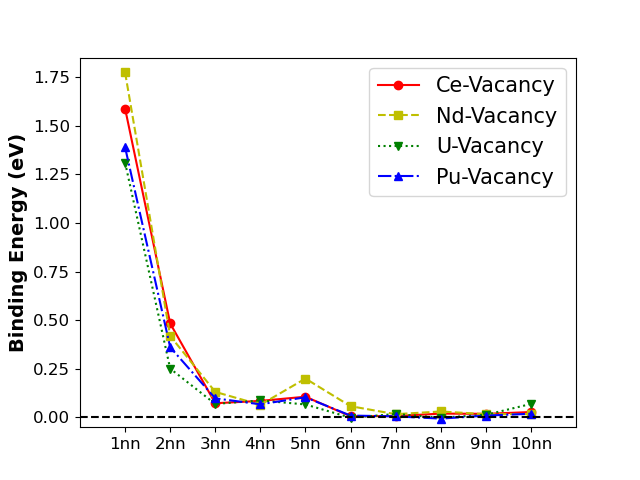
\includegraphics[width=0.99\linewidth]{BE.png}
    \caption{Solute-vacancy binding energies. The positive binding energies indicate attraction, and the negative binding energies indicate repulsion.}
    \label{fig:binding_energies}
\end{figure}

\begin{table}[h]
    \centering
    \caption{Notations, separation distances, orientations, and binding energies of vacancy-solute pairs considered in this work. Vacancy-solute distances (\textit{d}) are represented in terms of the lattice constant ($a_0$). The distances shown are between lattice sites in the unrelaxed crystal structure and are not the distances after the ionic relaxation. Results are compared with prior computational studies where available.}
    \begin{tabular}{|c|c|c|c|c|c|c|}
    \hline
       Notation & d ($a_0$) & Direction&  $E_{bind}^{sub-vac,Ce}$ & $E_{bind}^{sub-vac,Nd}$ &$E_{bind}^{sub-vac,U}$ &$E_{bind}^{sub-vac,Pu}$ \\
        \hline
       1nn &$\frac{\sqrt{3}}{2}$ & $<$1 1 1$>$ &1.588 eV &1.774 eV&1.310 eV&1.389 eV\\
       &&&1.87 \cite{yang_significant_2023} &1.70 \cite{yang_significant_2023} & & \\
       \hline
       2nn &1 & $<$1 0 0$>$ &0.483 eV&0.419 eV&0.251 eV&0.361 eV\\
       &&&0.48 \cite{yang_significant_2023} &0.35 \cite{yang_significant_2023} && \\
       \hline
       3nn &$\sqrt{2}$ &$<$1 1 0$>$  &0.073 eV&0.132 eV&0.070 eV&0.098 eV\\
       &&&0.12 \cite{yang_significant_2023} & 0.12 \cite{yang_significant_2023}&& \\
       \hline
       4nn &$\frac{\sqrt{11}}{2}$ & $<$3 1 1$>$ & 0.085 eV&0.065 eV&0.088 eV&0.068 eV\\
       &&&0.04 \cite{yang_significant_2023} &0.04 \cite{yang_significant_2023} && \\
       \hline
       5nn &$\sqrt{3}$ & $<$1 1 1$>$  & 0.107 eV&0.200 eV&0.067 eV&0.104 eV\\
       &&& &0.15 \cite{yang_significant_2023} && \\
       \hline
       6nn &2 & $<$1 0 0$>$ &0.006 eV&0.058 eV&-0.001 eV&0.010 eV\\
       \hline
       7nn &$\frac{\sqrt{19}}{2}$ & $<$3 3 1$>$ &0.007 eV&0.017 eV&0.018 eV&0.006 eV\\
       \hline
       8nn &$\sqrt{5}$ &$<$2 1 0$>$ &0.020 eV&0.031 eV&-0.001 eV&-0.006 eV\\
       \hline
       9nn &$\sqrt{6}$ & $<$2 1 1$>$  &0.019 eV&0.017 eV&0.014 eV&0.010 eV\\
       \hline
      10nn &$\frac{3\sqrt{3}}{2}$ & $<$1 1 1$>$ &0.028 eV&0.017 eV&0.069 eV&0.019 eV\\
      \hline
    \end{tabular}
    \label{tab:configurations_binding}
\end{table}

\FloatBarrier

All possible vacancy jumps from lattice sites within the 5nn shell—amounting to twelve distinct transitions—were evaluated using DFT. The vacancy jumps from the 1nn and the 2nn configurations are illustrated in \Cref{fig:jumps_all}. The jumps from the 3nn, 4nn, and 5nn configurations are illustrated in \Cref{fig:jumps_3nn_4nn} and \Cref{fig:jumps_5nn}. Notably, the solute-vacancy exchange jump (commonly referred to as $\omega_2$ in the nine-frequency model \cite{leclaire1970}) does not occur for the oversized solutes considered here. This behavior, also observed in BCC Fe by Bocquet \textit{et al.} \cite{bocquet_migration_2017} for Y and by Yang \textit{et al.} \cite{yang_significant_2023} for La, Ce, and Nd, arises because when the OSA occupies a 1nn site adjacent to a vacancy, it relaxes to an off-lattice site forming two half-vacancies, as shown in \Cref{fig:jumps_all}(a). As a result, the 1nn solute-vacancy exchange is prohibited.

\begin{figure}[!h]
    \centering
    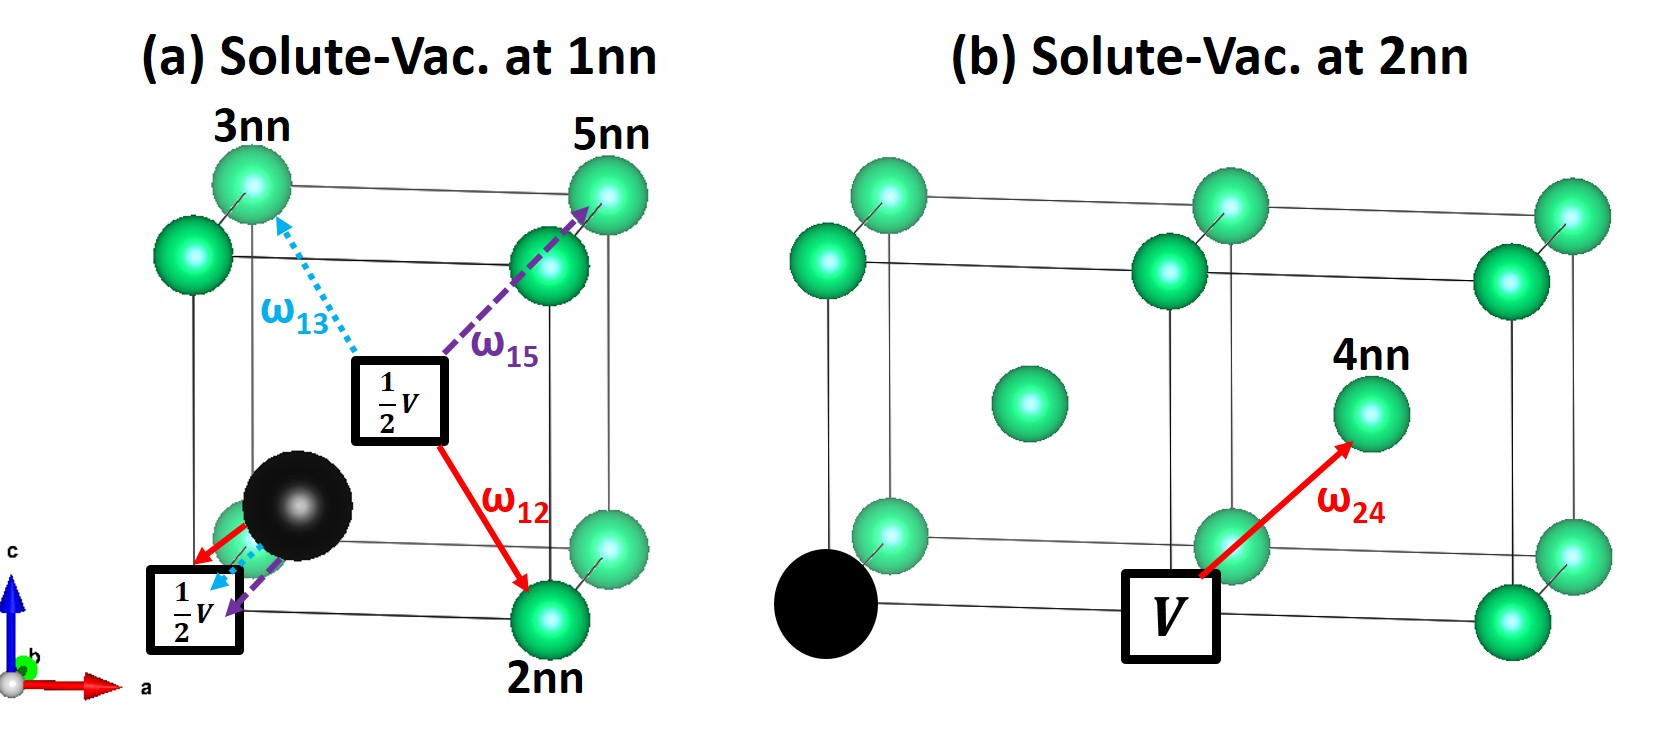
\includegraphics[width=0.8\linewidth]{jumps_Fe_1nn_2nn.jpg}
    \caption{(a) Schematic of the three possible jumps for a vacancy-solute pair initially in the 1nn configuration. The oversized solute atom (black sphere) is positioned between two half-vacancies. Each jump is labeled as $\omega_{if}$, where $i$ and $f$ indicate the initial and final configurations. In $\omega_{12}$, $\omega_{13}$, and $\omega_{15}$, the solute returns to its lattice site at the corner while the vacancy moves to the 2nn, 3nn, or 5nn site, respectively. (b) The jump ($\omega_{24}$) from the 2nn configuration.}
    \label{fig:jumps_all}
\end{figure}

\begin{figure}[h!]
    \centering
    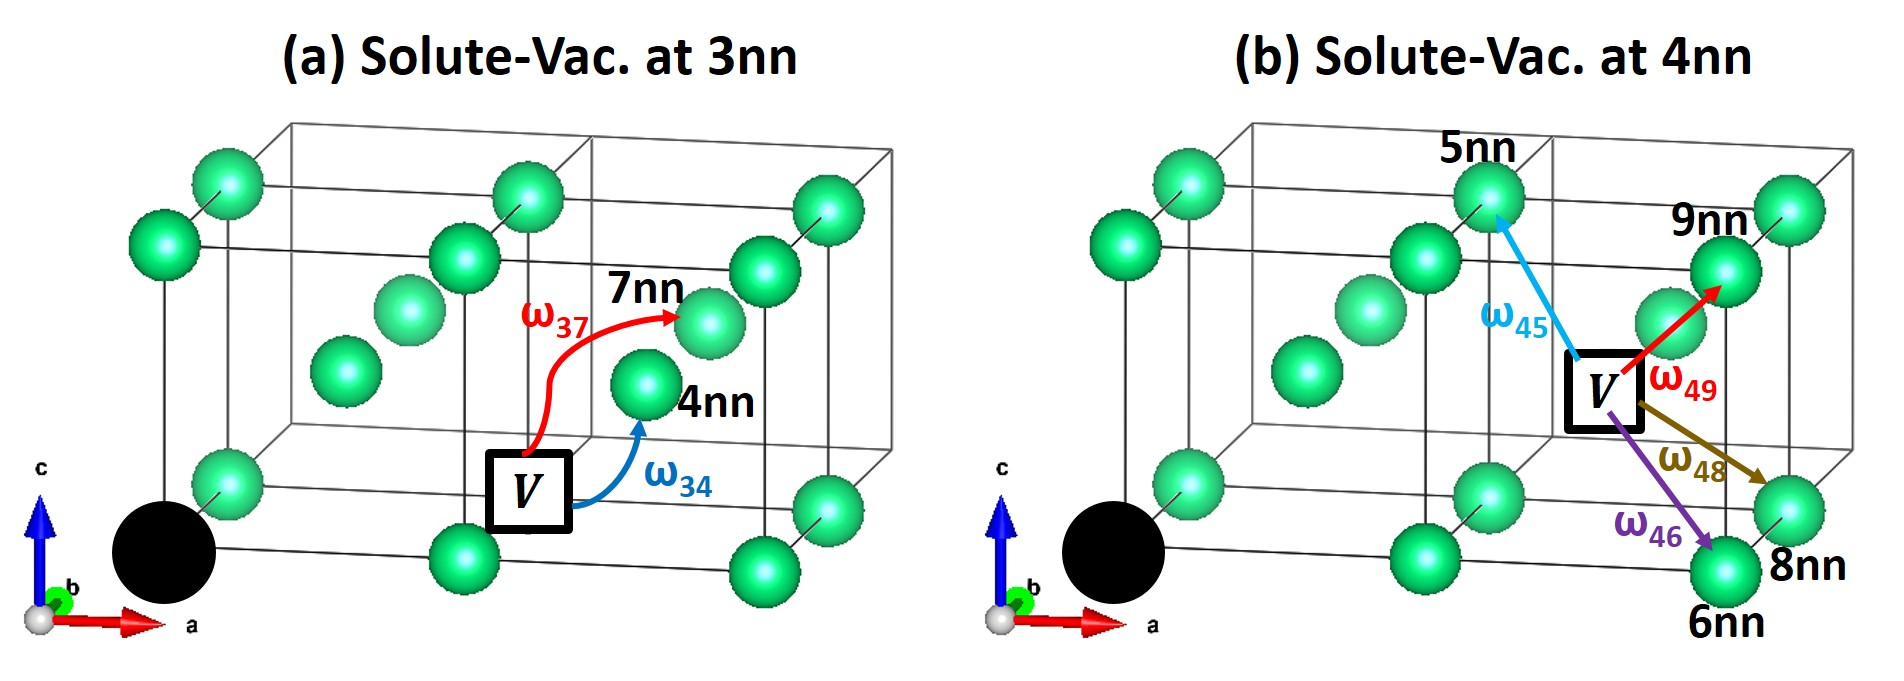
\includegraphics[width=0.95\linewidth]{3nn_and_4nn_jumps_fe.jpg}
    \caption{Schematic of possible vacancy jumps for vacancy-solute pairs in the (a) 3nn and (b) 4nn configurations. The jumps are labeled using the same notations of \Cref{fig:jumps_all}.}
    \label{fig:jumps_3nn_4nn}
\end{figure}

\begin{figure}[h!]
    \centering
    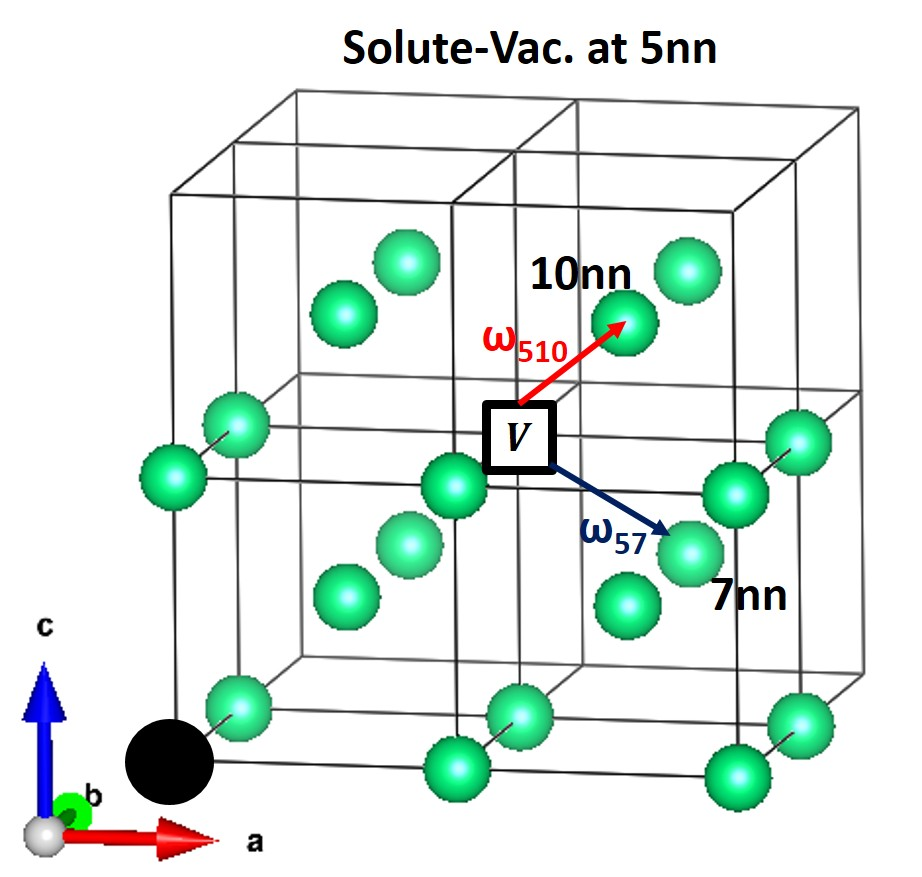
\includegraphics[width=0.5\linewidth]{5nn_jumps_fe.jpg}
    \caption{Schematic of the two possible vacancy jumps for a vacancy-solute pair in the 5nn configuration. The jumps are labeled using the same notation as \Cref{fig:jumps_all}.}
    \label{fig:jumps_5nn}
\end{figure}

\FloatBarrier

The complete set of migration barriers for the jumps is provided in \Cref{tab:migration_barriers}. The general trend is that lanthanides (Ce and Nd) have higher migration barriers than actinides (U and Pu). Overall, the results show good agreement with the prior DFT study of Yang \textit{et al.} \cite{yang_significant_2023} for Ce and Nd, with differences typically within 0.2–0.3 eV. The largest deviations are seen for the $\omega_{12}$ jump. The migration barriers for jumps $\omega_{15}$, $\omega_{57}$, and $\omega_{510}$ are left blank for the Nd and Ce cases. Our calculations indicate that the 5nn configuration is unstable for these solutes. Geometry optimizations for this configuration yield stable structures with attractive binding energies of 0.20 eV and 0.11 eV for Nd-vacancy and Ce-vacancy pairs, respectively. However, the CI-NEB calculations for the $\omega_{15}$ jump were unable to identify a saddle point. We explored the possibility of a very shallow barrier between the 1nn and 5nn states by increasing the number of intermediate images to 5, 7, and 9, but all results showed a monotonically increasing energy profile from the 1nn to the 5nn configuration. This suggests that the 5nn configuration is indeed unstable for Nd and Ce and will spontaneously relax to the 1nn configuration. This instability was also observed by Yang \textit{et al.} \cite{yang_significant_2023} for Ce in BCC Fe. Additionally, Yang \textit{et al.} reported a very shallow barrier, 0.02 eV above the 5nn configuration, for Nd in BCC Fe \cite{yang_significant_2023}.
For all vacancy jumps in bulk Fe listed in \Cref{tab:migration_barriers}, the attempt frequency of 11.6 THz \cite{messina_systematic_2016} in solute-free Fe is adopted for simplicity. This assumption will not affect the diffusion activation energies and will only affect the diffusion prefactors by less than one order of magnitude.



\begin{table}[!ht]
    \centering
    \caption{Migration barriers of $\omega_{ij}$ jumps in eV for bulk BCC Fe. The subscripts $i$ and $j$ denote the initial and final configurations, respectively. Results are compared with those of the prior computational study by Yang \textit{et al.} \cite{yang_significant_2023} where available.}
    \label{tab:migration_barriers}
    \begin{tabular}{|c|c|c|c|c|}
      \hline
      Jump &Ce &Nd &U  &Pu  \\
      \hline
       $\omega_{12}$  &1.951 &2.168 &1.748 &1.614 \\
       &2.48 \cite{yang_significant_2023}& 2.35 \cite{yang_significant_2023}&&\\
       \hline
       $\omega_{21}$  &0.847 &0.813 &0.689 &0.586 \\
       &1.09 \cite{yang_significant_2023}& 1.00 \cite{yang_significant_2023}&&\\
       \hline
       $\omega_{13}$  &1.738 &1.748 &1.632 &1.585 \\
       &1.89 \cite{yang_significant_2023}& 1.74 \cite{yang_significant_2023}&&\\
       \hline
       $\omega_{31}$  &0.223 &0.106 &0.391 &0.295 \\
       &0.14 \cite{yang_significant_2023}& 0.16 \cite{yang_significant_2023}&&\\
       \hline
       $\omega_{15}$  &- &- &1.430 &1.287 \\ 
       && 1.54 \cite{yang_significant_2023}&&\\
       \hline
       $\omega_{51}$  &- &- &0.187 &0.001 \\
       && 0.02 \cite{yang_significant_2023}&&\\
       \hline
       $\omega_{24}$  &0.824 &0.779 &0.728 &0.795 \\ 
       &0.84 \cite{yang_significant_2023} & 0.76 \cite{yang_significant_2023}&&\\
       \hline
       $\omega_{42}$  &0.426 &0.425 &0.564 &0.502 \\
       &0.40 \cite{yang_significant_2023} & 0.45 \cite{yang_significant_2023}&&\\
       \hline
       $\omega_{34}$  &0.724 &0.775 &0.698 &0.739 \\ 
       \hline
       $\omega_{43}$  &0.735 &0.708 &0.716 &0.708 \\
       \hline
       $\omega_{37}$ &0.672 &0.681 &0.672 &0.693 \\
       \hline
       $\omega_{73}$  &0.606 &0.567 &0.620 &0.600 \\
       \hline
       $\omega_{45}$ &0.690 &0.701 &0.652 &0.676 \\ 
       \hline
       $\omega_{54}$ &0.712 &0.836 &0.632 &0.712 \\
       \hline
       $\omega_{46}$ &0.751 &0.725 &0.746 &0.730 \\
       \hline
       $\omega_{64}$ &0.672 &0.718 &0.657 &0.672 \\
       \hline
       $\omega_{48}$ &0.701 &0.695 &0.701 &0.701 \\ 
       \hline
       $\omega_{84}$  &0.636 &0.661 &0.612 &0.627 \\
       \hline
       $\omega_{49}$ &0.689 &0.687 &0.681 &0.679 \\ 
       \hline
       $\omega_{94}$  &0.622 &0.639 &0.608 &0.621 \\
       \hline
       $\omega_{57}$ &- &- &0.677 &0.696 \\ 
       \hline
       $\omega_{75}$  &- &- &0.628 &0.598 \\
       \hline
       $\omega_{510}$ &- &- &0.654 &0.687 \\ 
       \hline
       $\omega_{105}$  &- &- &0.656 &0.602 \\
       \hline
    \end{tabular}
\end{table}



\FloatBarrier
\subsection{Corrections to Arrhenius Diffusion in Bulk Fe}

\noindent The DFT-calculated energetics in the previous section are used as input to KineClue \cite{schuler_kineclue_2020} to evaluate the transport coefficients and solute diffusivities. The evaluated diffusivities ($D$) may be fitted to an Arrhenius expression:
\begin{equation}
    D = D_0 e^{\frac{-Q_0^F}{k_B T}},
\end{equation}
where $Q_0^F$ is the activation energy and $D_0$ is the prefactor. This expression is valid at low temperatures well below the Curie temperature of $T_C$ = 1043 K, at which the transition to the paramagnetic state occurs. Diffusion experiments \cite{lubbehusen1990self, hettich1977self} show that at high temperatures closer to $T_C$, magnetic disordering leads to a significant change in the activation energies. Furthermore, it was shown that a non-negligible contribution of electronic excitations plays a role in the diffusion activation energy in BCC metals \cite{satta1998vacancy, sandberg2015modeling}. To include these finite-temperature effects, the corrected activation energy, $Q(T)$, can be written as:
\begin{equation}
\label{eq:corrected_Q}
    Q(T) = Q_0^F + Q_2T^2 -\alpha H(T),
\end{equation}
where $Q_2T^2$ is the correction for electronic excitations, and the value of $Q_2$ is assumed to be $1.1 \times 10^{-7} eV/K^2$ as calculated by Sandberg \textit{et al.} \cite{sandberg2015modeling}. The $\alpha H(T)$ term is the magnetic disordering correction following the approach discussed in references \cite{messina_systematic_2016, jonsson1992ferromagnetic}. The $H(T)$ factor is the magnetic excess enthalpy as a function of temperature normalized by the magnetic excess enthalpy at 0 K. The expression used for $H(T)$ in this work was derived by J\"{o}nsson \cite{jonsson1992ferromagnetic} using the Hillert--Jarl semi-empirical model \cite{hillert1978model}:
\begin{equation}
    H(T)=\frac{120}{71}(1-P)(\frac{\tau^{4}}{2}+\frac{\tau^{10}}{15}+\frac{\tau^{16}}{40}),
\end{equation}
where $\tau$ is $T/T_C$, and $P$ is a geometry factor and is 0.4 for BCC \cite{jonsson1992ferromagnetic}. The parameter $\alpha$ is the difference between the activation energies of the ferromagnetic and paramagnetic states ($\alpha = Q^F_0-Q^P$). Using the calculated values for $Q^F_0$ and $Q^P$ by Sandberg \textit{et al.}\cite{sandberg2015modeling} yields $\alpha = 0.87$ eV.
Applying these corrections in \Cref{eq:corrected_Q}, the self-diffusivity is plotted in \Cref{fig:self_diff}  with experimental data from references \cite{lubbehusen1990self, hettich1977self}. The correction is considered negligible at low temperatures below 650 K ($1/T > 1.54 \times 10^{-3}$ K$^{-1}$), as seen in \Cref{fig:self_diff}. At high temperatures, the introduced corrections deviate the diffusivities from the Arrhenius behavior and bring our results into good agreement with experimental results. 

\begin{figure}[!ht]
    \centering
    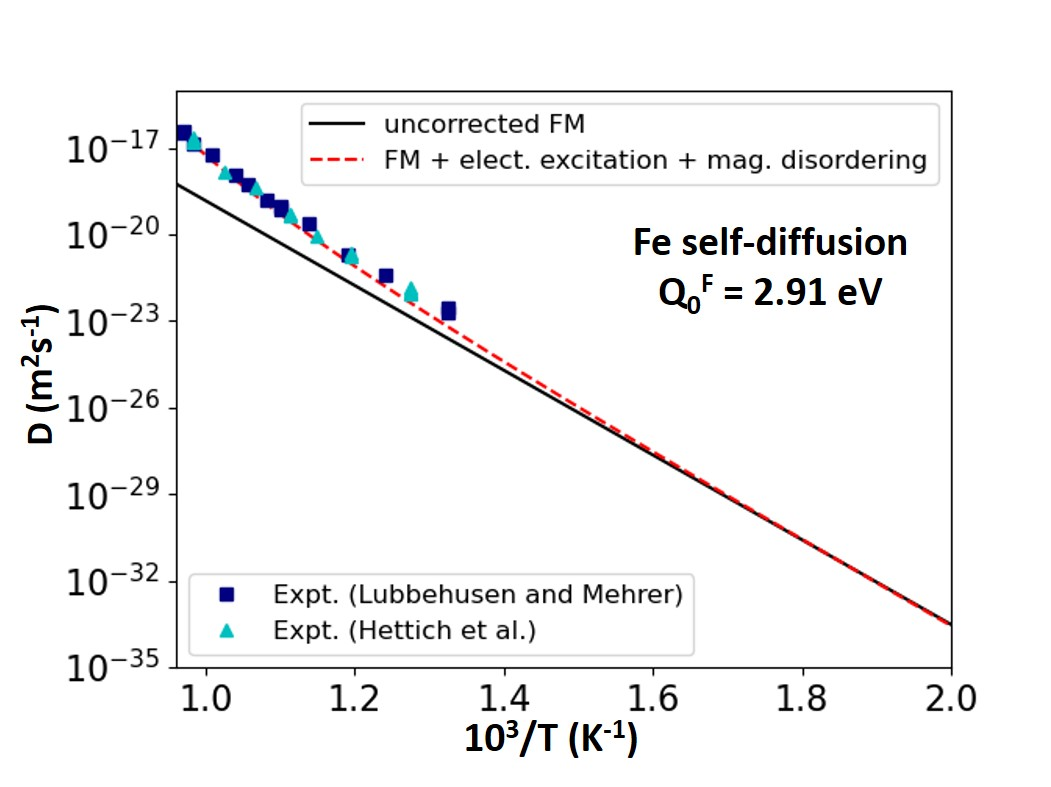
\includegraphics[width=0.8\linewidth]{self_diffusivity.jpg}
    \caption{The self-diffusivity in bulk BCC Fe is plotted versus inverse temperature. The $Q_0^F$ value is the diffusion activation energy for the uncorrected ferromagnetic results (black solid lines). The corrected diffusivity, including contributions from electronic excitations and finite-temperature magnetic disordering, is plotted in a red dashed line. Experimental data from references \cite{lubbehusen1990self, hettich1977self} are shown for comparison.}
    \label{fig:self_diff}
\end{figure}

The calculated self-diffusion coefficients in BCC Fe exhibit a slope (activation energy, $Q_0^F$) that closely matches that of the experimental self-diffusion data reported in \cite{lubbehusen1990self, hettich1977self} (see \Cref{tab:activation_energies} for values of $Q_0^F$). This close agreement supports the reliability of the DFT-computed defect energetics and the validity of the vacancy-mediated diffusion mechanism assumed in this work.

\subsection{Lanthanide and Actinide Diffusion in Bulk Fe}

The same corrections described in \Cref{eq:corrected_Q} are applied to solute diffusivities via the vacancy mechanism in the dilute limit, under the assumption that a single solute atom has a negligible impact on the correlation between the magnetic state and vacancy migration properties. The solute diffusivities, both with and without these corrections, are shown in \Cref{fig:diff_Q}. Ce, Nd, U, and Pu all diffuse faster than the Fe self-diffusion, which is shown in \Cref{fig:self_diff}. Among these elements, Nd exhibits the highest diffusivity with an activation energy of 2.20 eV, while U diffuses the slowest, with an activation energy of 2.57 eV. 

%Ce and Nd have an almost temperature-independent correlation factor of  0.3-0.4. U and Pu have correlation factors that are strongly temperature-dependent. dependent (1e-4 at low T to 0.2 at high T). Not sure about the explanation for this. Probably because U and Pu have more competing jump pathways 1-2, 1-3, and 1-5 with comparable saddle point energies. Temperature affects which jump dominates. For Ce and Nd: jump 1-3 is always more dominant. Not sure if this is worth mentioning.

\begin{figure}[!ht]
    \centering
    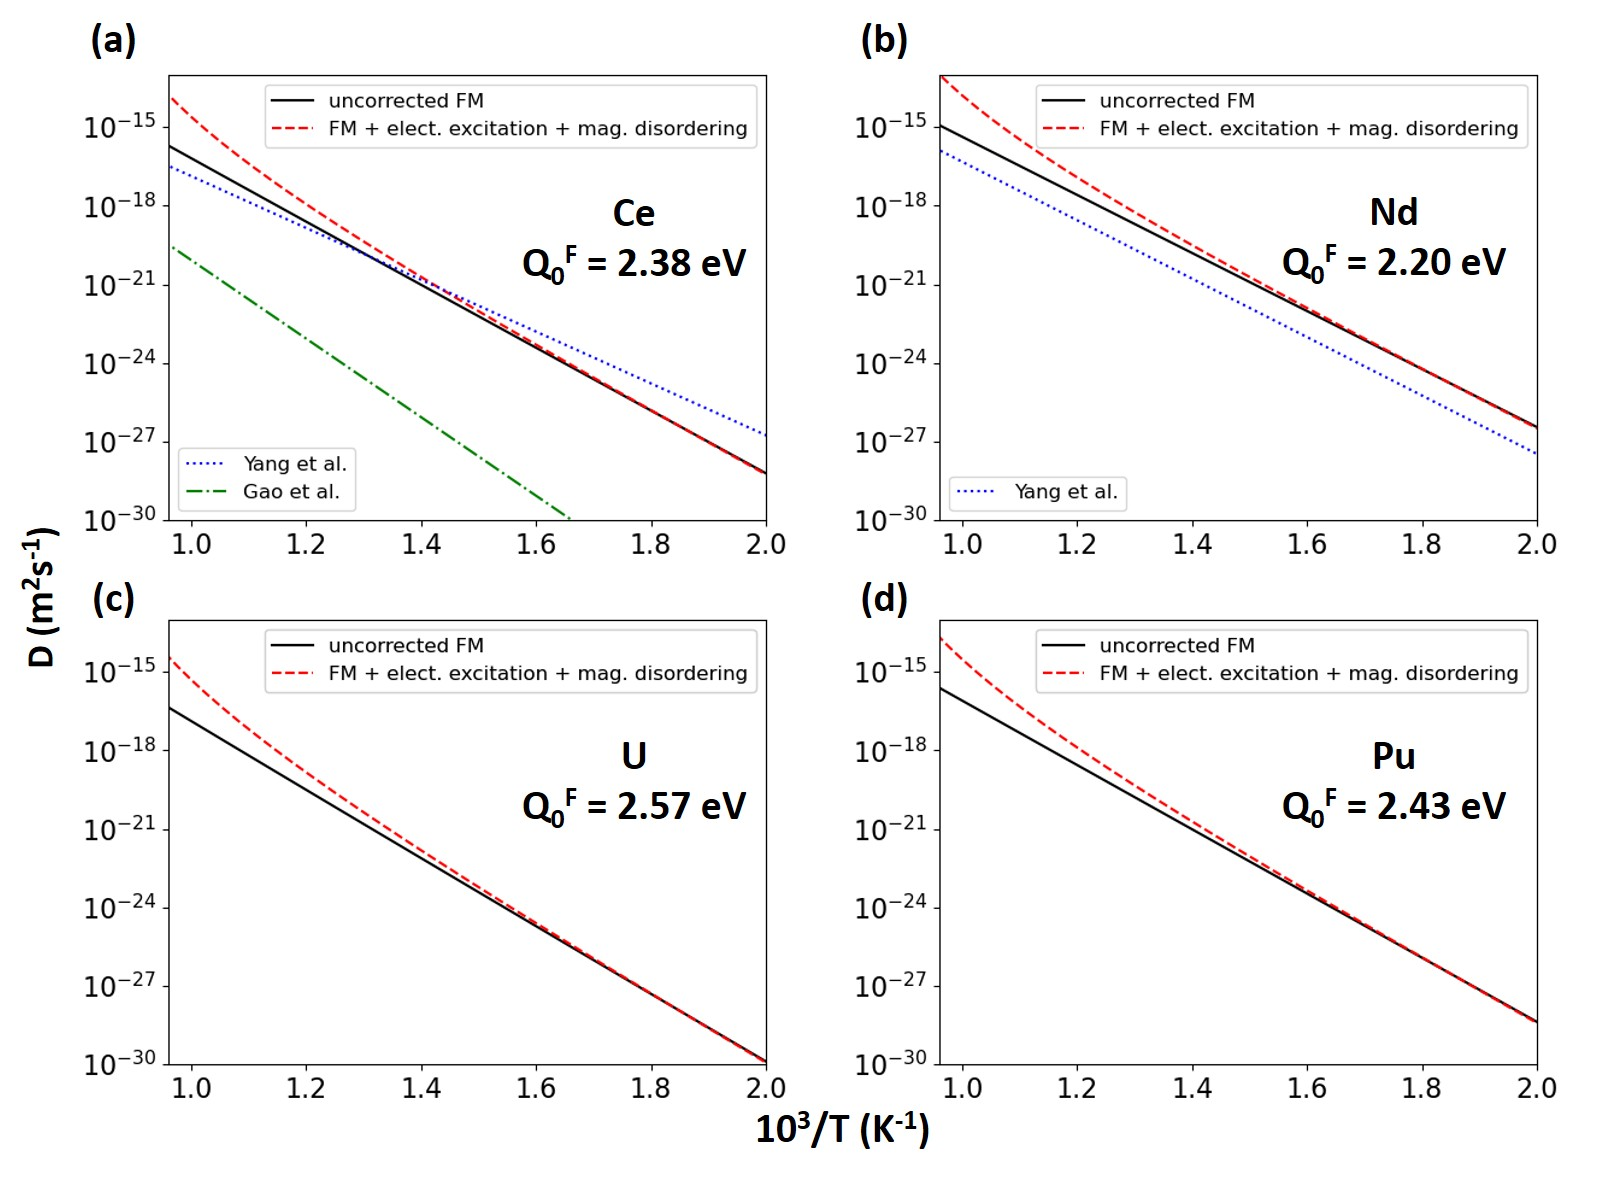
\includegraphics[width=\linewidth]{diffusivities_Q.jpg}
    \caption{The diffusivities of (a) Ce, (b) Nd, (c) U, and (d) Pu in bulk BCC Fe are plotted versus inverse temperature. The $Q_0^F$ values are the diffusion activation energies for the uncorrected ferromagnetic results (black solid lines). The corrected diffusivities, including contributions from electronic excitations and finite-temperature magnetic disordering, are plotted in red dashed lines. Results from references \cite{yang_significant_2023, GAO2016316} are shown for comparison.}
    \label{fig:diff_Q}
\end{figure}


It is important to note that the relatively high migration barriers for vacancy-solute exchange, reported in \Cref{tab:migration_barriers}, do not contradict the observation that these solutes diffuse faster than Fe. These solutes diffuse faster because they experience strong vacancy drag due to their substantial attractive binding energies with vacancies, which enhances their diffusivity. To quantify this effect, the off-diagonal transport coefficients are utilized to evaluate the vacancy drag ($G_V$) and partial diffusion coefficient ($D_{pd}$) ratios. The results reveal that lanthanides and actinides are strongly dragged by vacancies. As shown in \Cref{fig:vacancy_drag}(a), all species except U exhibit \( G_V \approx 1 \), indicating strong kinetic coupling between solute and vacancy fluxes. Consequently, \( D_{pd} \) remains negative (see \Cref{fig:vacancy_drag}(b)), suggesting solute enrichment at sinks across all temperatures. For U, \( G_V \) decreases with temperature, from 1 at 300~K to 0.5 at 1000~K, but no transition to the IKE regime (\( G_V < 0 \)) is observed, unlike with other solutes in BCC Fe such as transition metals (Cu, Ni, and Mn)  \cite{messina_exact_2014, messina_solute_2020}.
This behavior is attributed to the strong attractive binding between lanthanides or actinides and vacancies. These oversized solutes exhibit high vacancy binding energies of 1.30–1.80~eV at the 1nn compared to only 0.1–0.3~eV for Cu, Ni, and Mn, as reported by Messina \textit{et al.}~\cite{messina_exact_2014}.


\FloatBarrier

\begin{figure}[!ht]
    \centering
    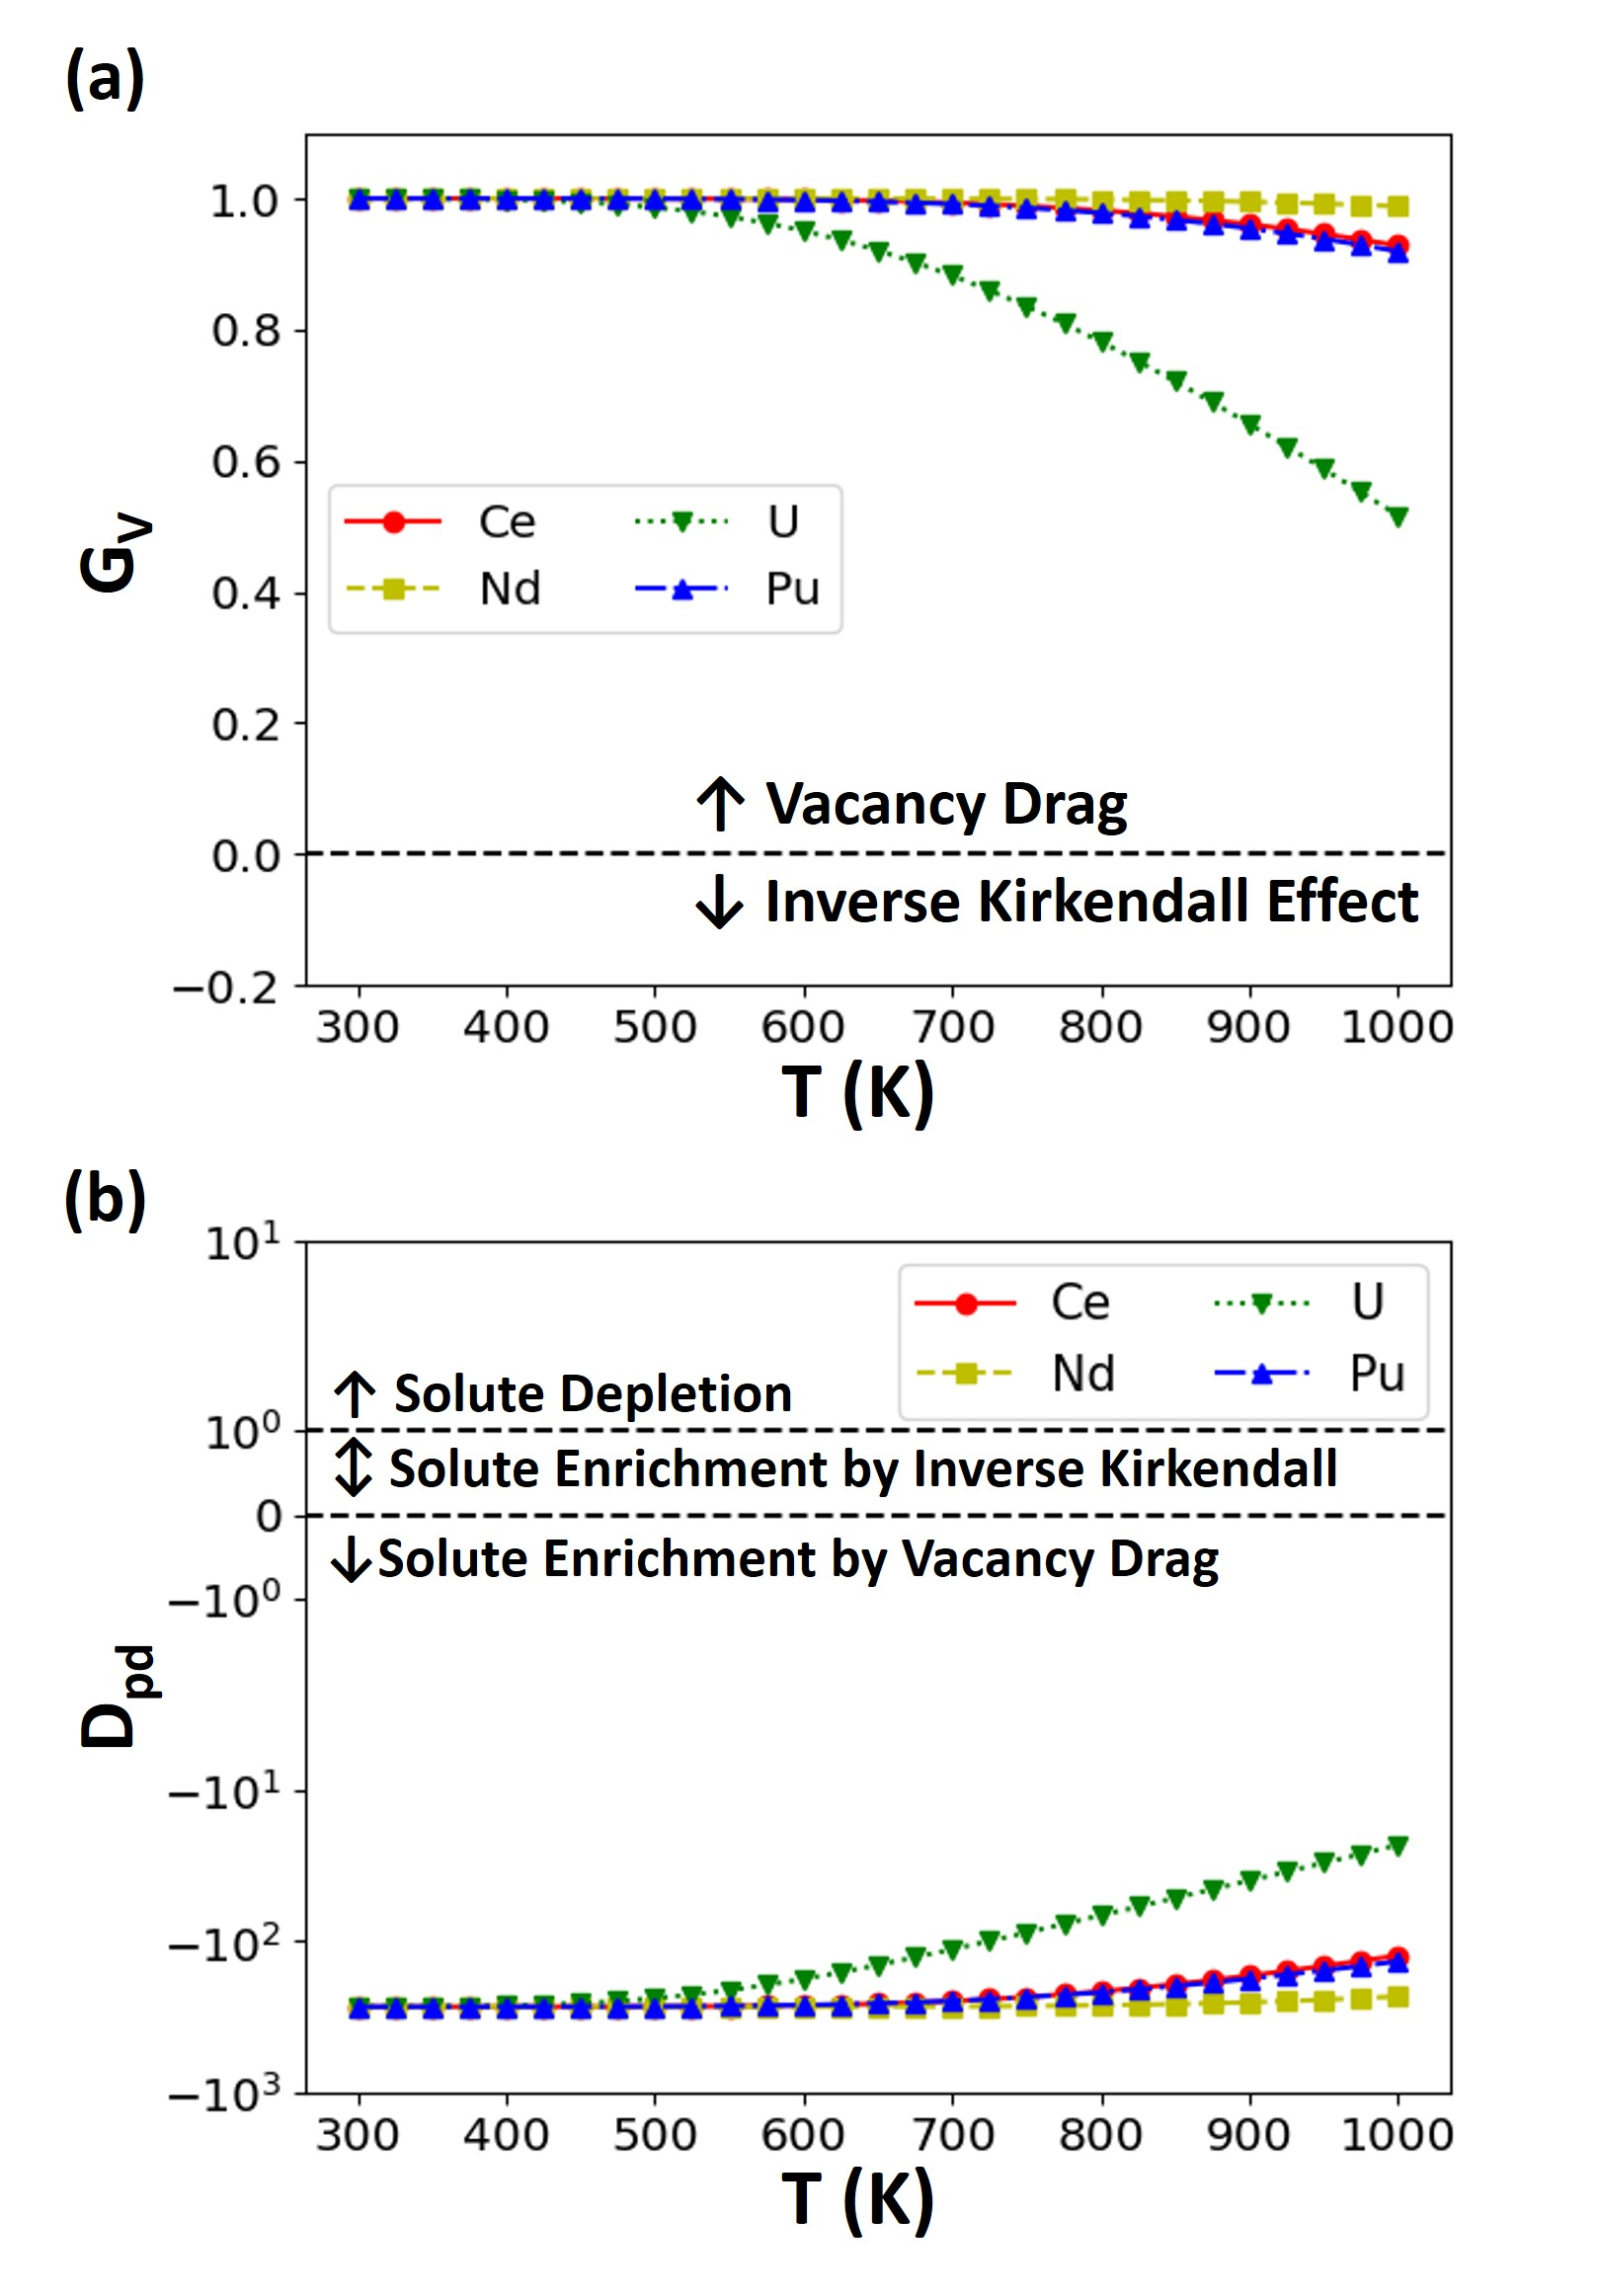
\includegraphics[width=0.625\linewidth]{drag_ratios_pdc_fe.jpg}
    \caption{(a) Vacancy drag ratios ($G_V$) and (b) partial diffusion coefficient ratios ($D_{pd}$) plotted versus temperature.}
    \label{fig:vacancy_drag}
\end{figure}


\Cref{tab:activation_energies} summarizes the fitted activation energies in the ferromagnetic regime, $Q_0^F$, and the diffusion prefactors, $D_0$, compared to those of previous DFT studies \cite{yang_significant_2023,sandberg2015modeling, GAO2016316} and the experimental fit \cite{lubbehusen1990self}. 
The diffusion activation energy of Nd in BCC Fe obtained in this study agrees well with the DFT results reported by Yang \textit{et al.} \cite{yang_significant_2023}, as shown in \Cref{fig:diff_Q}(b) and \Cref{tab:activation_energies}. However, our results exhibit a slight upward shift relative to those of Yang \textit{et al.} due to the different attempt frequencies used for Nd-vacancy jumps. For Ce, Yang \textit{et al.} \cite{yang_significant_2023} and Gao \textit{et al.} \cite{GAO2016316} reported activation energies that differed significantly, by about 1 eV, as seen in \Cref{fig:diff_Q}(a) and \Cref{tab:activation_energies}. Our results are in better agreement with those of Yang \textit{et al.} \cite{yang_significant_2023}. 
As of this writing, and to the best of our knowledge, no prior computational studies exist for U and Pu for comparison. 
In \Cref{sec:discussion1}, we present an analysis of the differences in Ce diffusivities from various sources and compare our solute diffusivities with experimental data.


\begin{table}[!ht]
    \centering
    \caption{Activation energies and prefactors for self-diffusion and solute diffusion in bulk BCC Fe via the vacancy mechanism. The activation energies $Q_0^F$ are valid for low temperatures well below $T_C$. At high temperatures, the corrections in \Cref{eq:corrected_Q} must be applied.}
    \label{tab:activation_energies}
    \begin{tabular}{|c|c|c|c|c|c|c|}
    \hline
         &&Fe tracer&Ce&Nd&U&Pu  \\
    \hline
    This Work& $Q_0^F$ (eV)&2.91&2.38&2.20&2.57&2.43 \\
                &  $D_0$ ($\times 10^{-6} m^2 s^{-1}$)
    &68.7&60.7&48.5&108.1&140.8\\
    \hline
    DFT&$Q_0^F$ (eV)
    & 2.87\cite{sandberg2015modeling} &1.96\cite{yang_significant_2023},2.97\cite{GAO2016316}
    &2.21\cite{yang_significant_2023}&-&-\\
                &$D_0$ ($\times 10^{-6} m^2 s^{-1}$)
    &84.6\cite{sandberg2015modeling}
    &0.1\cite{yang_significant_2023}, 7.7\cite{GAO2016316}
    &6.4\cite{yang_significant_2023}&-&-\\
    \hline
    Experiments &$Q_0^F$ (eV)& 2.87\cite{lubbehusen1990self}
    &-&-&-&- \\
                &  $D_0$ ($\times 10^{-6} m^2 s^{-1}$)& 66.0\cite{lubbehusen1990self} &-&-&-&- \\
    \hline
    \end{tabular}
\end{table}


\FloatBarrier
\subsection{Point Defects on Fe Surface}

\noindent First, the segregation energies \( E_{\text{seg}}\) for vacancies and substitutional solutes (Ce, Nd, U, and Pu) on the (110) surface of BCC Fe are evaluated. The surface is modeled using a slab consisting of six atomic layers, which provide three symmetry-inequivalent vacancy or substitutional sites within the top three layers from either free surface, as illustrated in \Cref{fig:surface_seg}(a). These sites allow us to assess the defect preference as a function of depth from the surface.. The (110) surface is chosen because it is the most densely packed and the lowest energy surface in BCC Fe \cite{tran2016surface}, making it the most stable and relevant for surface diffusion studies.

\begin{figure}[!ht]
    \centering
    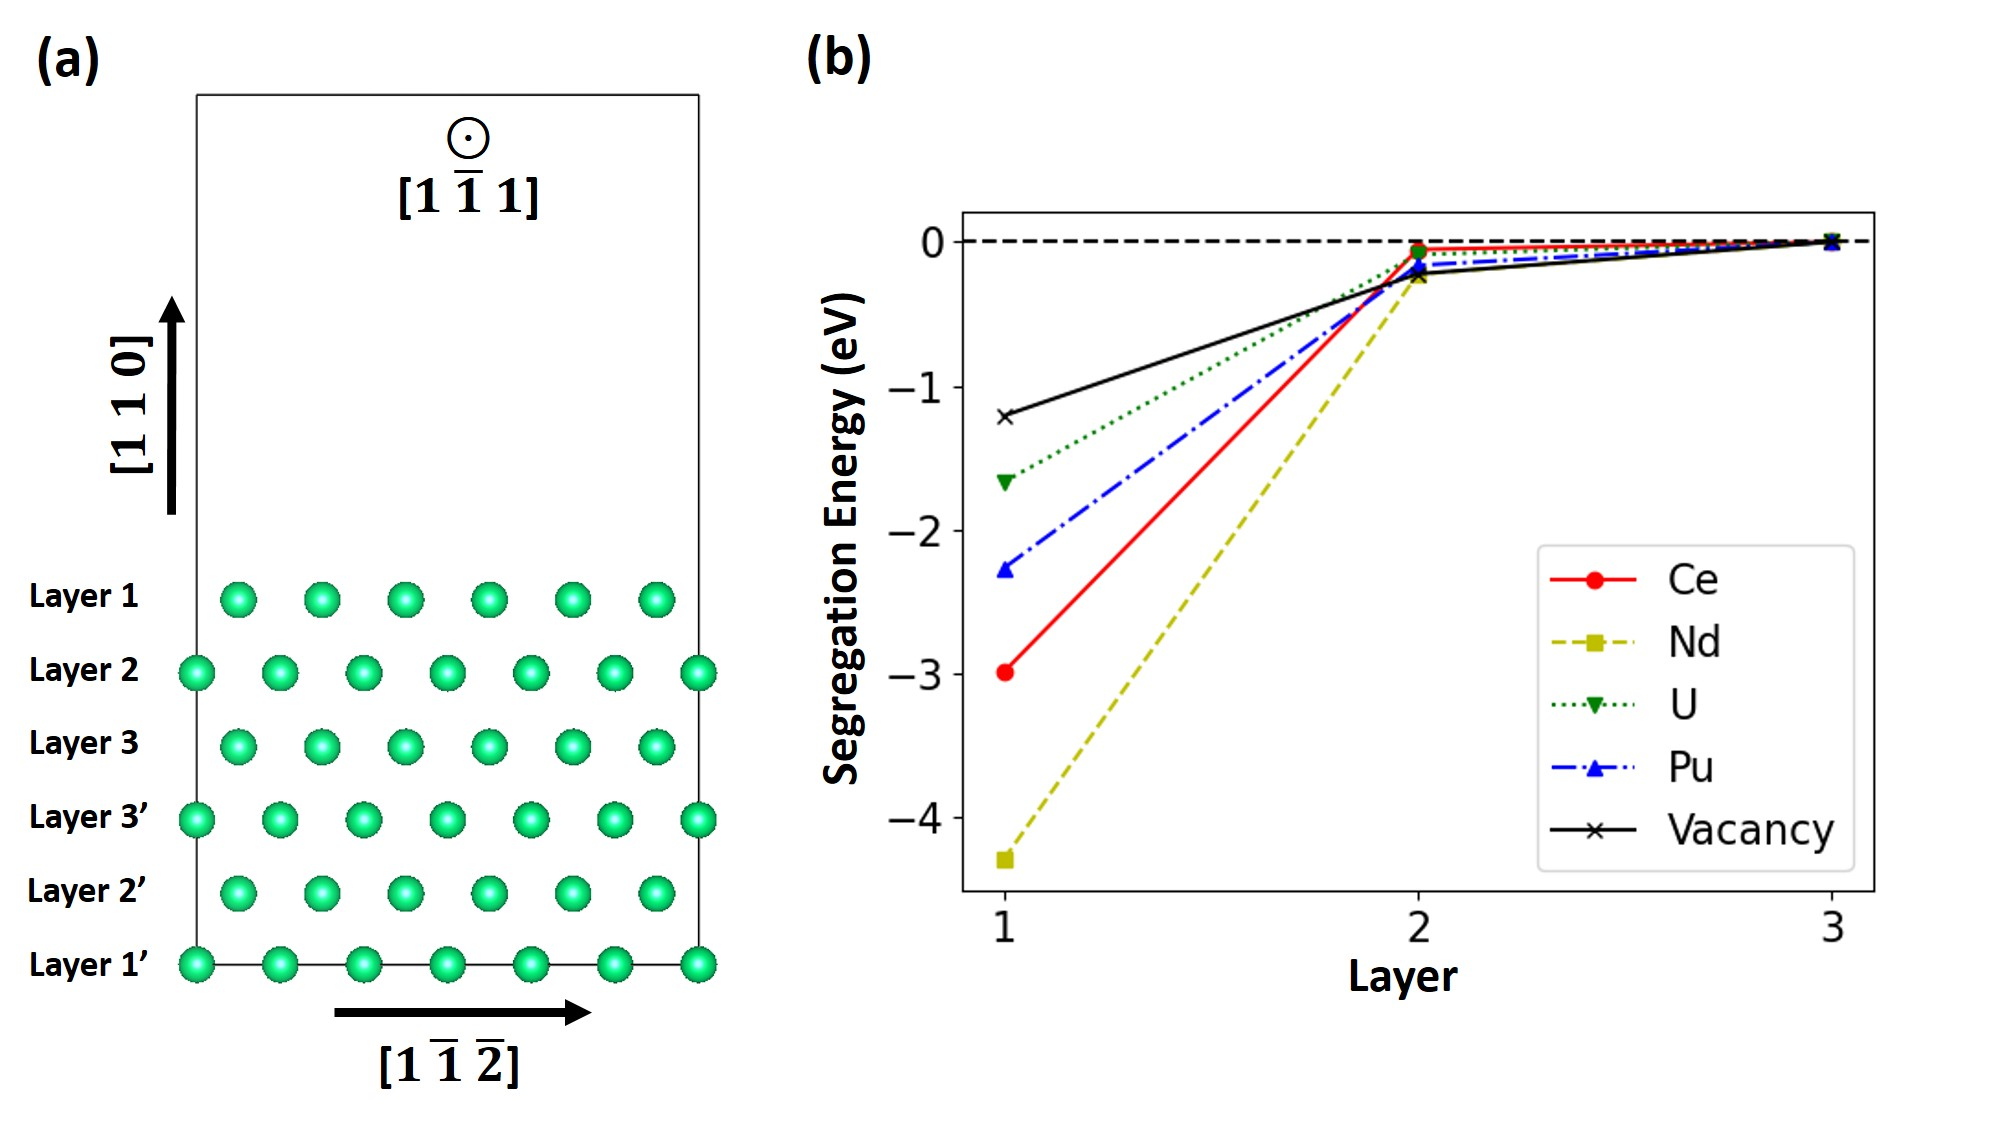
\includegraphics[width=\linewidth]{seg_surface.jpg}
    \caption{(a) Side view of the slab used in the (110) surface calculations where the [$1\overline{1}1$] direction is perpendicular to the page. (b) The segregation energies of vacancies and substitutional solutes on the (110) surface in BCC Fe are plotted for the first three layers from the surface. }
    \label{fig:surface_seg}
\end{figure}

%at thermodynamic equilibrium and in dilute limit : segregation factor s = exp(-E_seg/kT) = C_solute_surface/C_solute_bulk

The segregation energy quantifies the thermodynamic force that drives a vacancy or solute atom to migrate from a bulk-like environment to a surface or near-surface site. It is defined as:
\begin{equation}
    E_{\text{seg}}^{\text{defect},i} = (E_{\text{defect}}^{\text{i}})_{\text{surface}} - (E_{\text{defect}}^{\text{i}})_{\text{bulk}},
\end{equation}

\noindent where \( (E_{defect}^{i})_{surface} \) and \( (E_{defect}^{i})_{bulk} \) represent the DFT energies of supercells with a defect $i$ at a surface (or near-surface) site and a bulk-like reference site, respectively. To maintain consistency within the computational framework, we used the third atomic layer of the slab as the bulk reference site instead of performing separate bulk calculations. This approach mitigates potential discrepancies arising from supercell size and \( k \)-point sampling differences between slab and bulk models, thereby enabling a more robust and internally consistent comparison of formation energies.

The resulting segregation energies are presented in \Cref{fig:surface_seg}(b). All four solutes exhibit a strong thermodynamic preference for occupying the first surface layer, which indicates significant surface segregation tendencies. Among them, Nd shows the strongest segregation with an energy of \( -4.30 \) eV, followed by Ce, Pu, and U, with U exhibiting the weakest (yet still substantial) segregation energy of \( -1.67 \) eV. These negative values reflect the energetic stabilization of solutes at the surface relative to the bulk, implying that once a lanthanide or actinide atom reaches the surface, particularly the outermost layer, it is highly unlikely to diffuse back into the bulk. Similarly, vacancies exhibit a strong segregation with an energy of -1.21 eV at the outermost layer. Consequently, for this study, surface diffusion is assumed to be confined to two-dimensional motion within the first atomic layer. This two-dimensional diffusion of vacancies on the first layer of an Fe (110) surface was also reported by a molecular dynamics (MD) study \cite{wang2010single} as the dominant diffusion mechanism. Adatom diffusion on Fe surfaces may also play a role, as suggested by Wang \textit{et al.} \cite{wang2012molecular}.

Given that the primary objective is to use surface diffusivities as a surrogate for GB diffusivities, our analysis focuses exclusively on vacancy-mediated diffusion mechanisms. This is motivated by prior experimental and computational studies that indicate that vacancy diffusion is a dominant mechanism for impurity and self-diffusion along Fe GBs \cite{balluffi1982grain,peterson1983grain, klotsman1990impurity, kwok1981, inoue2007grain}. As such, alternative mechanisms, such as adatom diffusion, are excluded from consideration in this work.

Similar to the bulk diffusion analysis, solute-vacancy binding and migration energies are calculated on the (110) surface within a defined thermodynamic interaction range. To reduce computational cost, the analysis is restricted to vacancy jumps from the 1nn and 2nn configurations, omitting jumps from the 3nn to 5nn configurations that were included in the bulk Fe study. The solute-vacancy configurations and jumps considered on the surface are illustrated in \Cref{fig:binding_mig_surface}(a).

\begin{figure}[!ht]
    \centering
    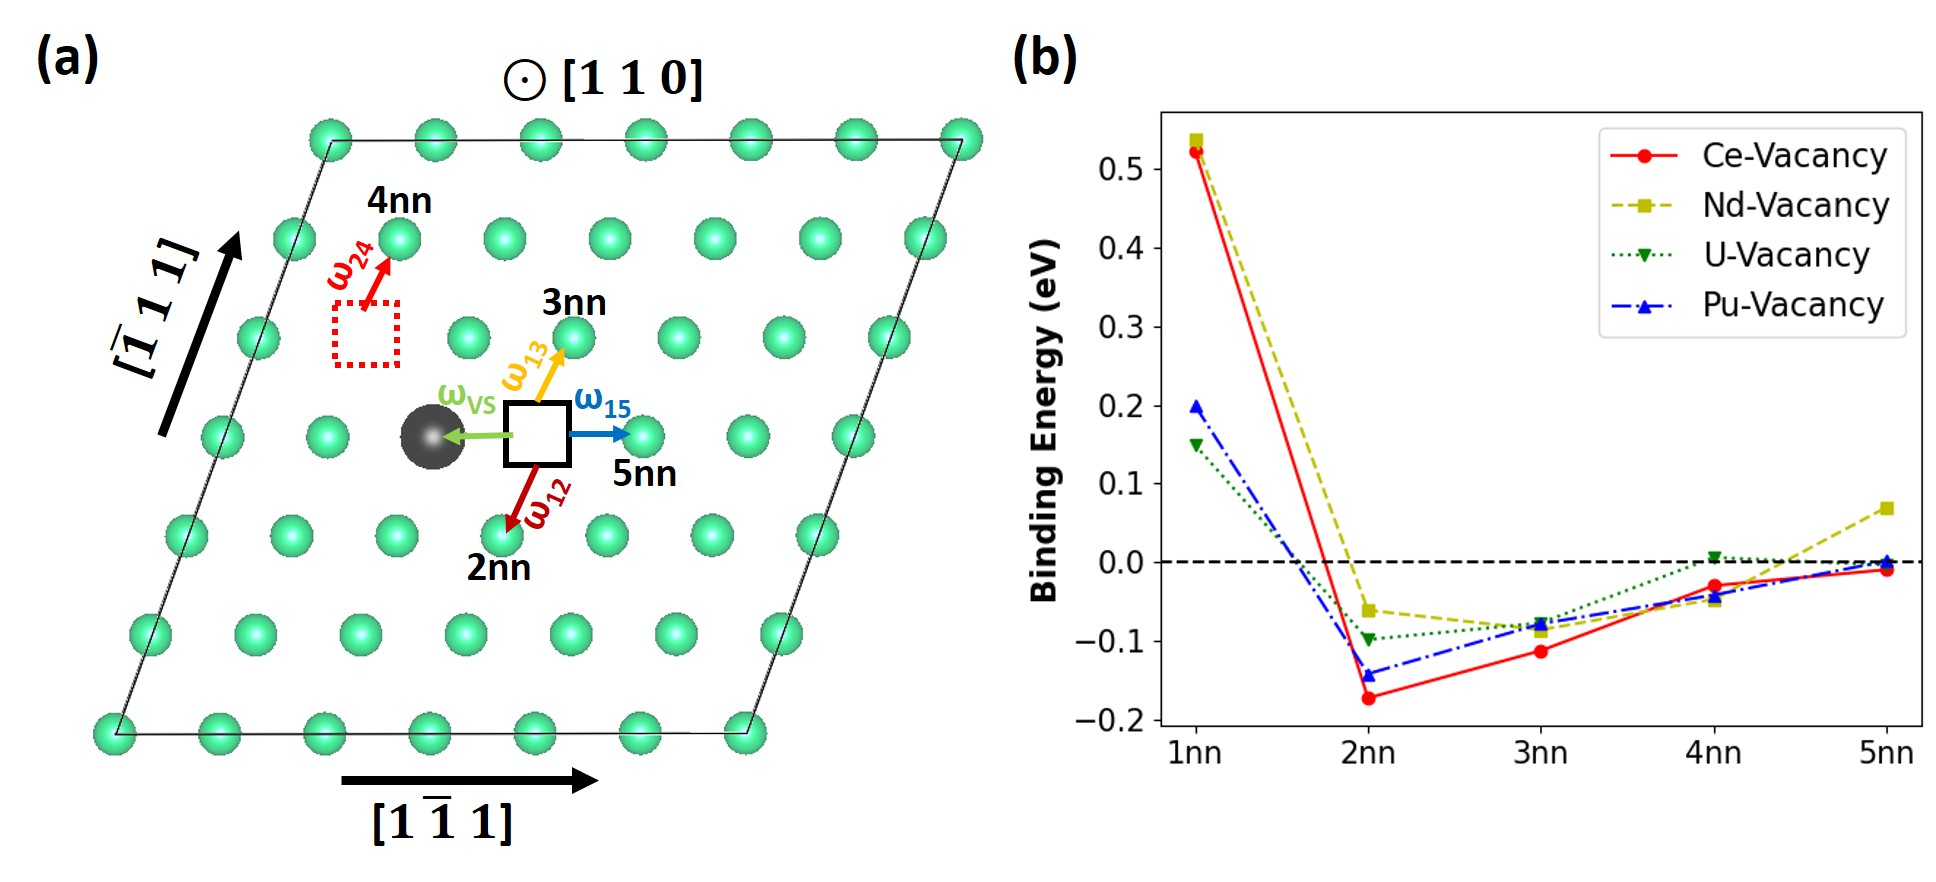
\includegraphics[width=\linewidth]{bind_surface.jpg}
    \caption{(a) Top view of layer 1 of the (110) surface showing the solute-vacancy interactions and vacancy jumps considered. The solute atom is shown in a black sphere, while the hollow square represents a vacancy at the 1nn (solid black square) and 2nn (dotted red square) configurations. (b) Solute-vacancy binding energies on the (110) surface (layer 1) are plotted for up to the 5nn configuration. Positive binding energy indicates attraction, while negative binding energy indicates repulsion.}
    \label{fig:binding_mig_surface}
\end{figure}

\Cref{fig:binding_mig_surface}(b) shows the calculated solute-vacancy binding energies for configurations up to the 5nn. Notably, the two-half-vacancy configuration at the 1nn—observed in bulk Fe for all solutes—was only found for U on the surface and was absent for Ce, Nd, and Pu. As a result, the vacancy-solute exchange jump ($\omega_{VS}$, also known as $\omega_2$ in the nine-frequency model \cite{leclaire1970}) is specifically considered and included in the surface jump configurations shown in \Cref{fig:binding_mig_surface}(a), except for U.
The binding energy trends in \Cref{fig:binding_mig_surface}(b) indicate attractive interactions at the 1nn and repulsive interactions at the 2nn and 3nn for all four solutes. At the 4nn and 5nn, the binding energies generally approach zero (within $\pm$0.05 eV), indicating negligible interaction, except for the Nd-vacancy pair at the 5nn, which shows a slightly attractive binding energy of 0.07 eV. This was also observed for the Nd-vacancy at the 5nn configuration in the bulk system, as shown in \Cref{fig:binding_energies}.

The equilibrium concentration of vacancies (\( C_V \)) on the outermost layer of the (110) surface is calculated using \Cref{eq:conc_vac}, based on the computed vacancy formation energy and entropy, \( E_{\text{form}}^{\text{vac}} = 1.22 \)~eV and \( S_{\text{form}}^{\text{vac}} = 2.1\,k_B \), respectively. Both values are notably lower than their counterparts in bulk Fe, as listed in \Cref{tab:bulk_properties}. The vacancy migration barriers are summarized in \Cref{tab:mig_barriers_surface}. In a solute-free slab, the vacancy migration energy \( E_{\text{mig}}^{\text{vac}} \) is calculated to be 0.621~eV, which is used to estimate the surface self-diffusivity of an Fe tracer atom. Interestingly, this barrier is comparable to the bulk value of 0.69~eV, indicating that vacancy mobility on the surface is similar to that in the bulk. This similarity was also reported by Kochaev and L'vov \cite{kochaev2024atomistic}, who found that the calculated vacancy migration barriers along the Fe $\Sigma3$(112) GB were 0.57–0.61 eV compared to 0.64 eV for the bulk. Thus, the enhancement in vacancy-mediated diffusion on the (110) surface compared to bulk diffusion is driven by a significantly higher vacancy concentration on the surface because \( E_{\text{form}}^{\text{vac}} \) is approximately 1~eV lower than it is in the bulk.


\begin{table}[!ht]
    \centering
    \caption{Migration barriers in eV for the vacancy-solute exchange, $\omega_{VS}$, and the $\omega_{ij}$ jumps on the (110) surface of BCC Fe shown in \Cref{fig:binding_mig_surface}(a). The subscripts $i$ and $j$ denote the initial and final configurations, respectively. }
    \begin{tabular}{|c|c|c|c|c|c|}
      \hline
      Jump &Fe tracer& Ce & Nd & U & Pu \\
      \hline
      $\omega_{VS}$&0.621&0.054 &0.021 &- &0.086  \\
      \hline
      $\omega_{12}$&-&0.983 &1.141 &0.621 &0.827 \\
      $\omega_{21}$&-&0.288 &0.542 &0.374 &0.486 \\
      \hline
      $\omega_{13}$&-&0.907 &0.841 &0.621 &0.672 \\
      $\omega_{31}$&-&0.271 &0.218 &0.395 &0.394 \\
      \hline
      $\omega_{15}$&-&0.650 &0.558 &0.600 &0.539 \\
      $\omega_{51}$&-&0.117 &0.090 &0.447 &0.341 \\ 
      \hline
      $\omega_{24}$&-&0.370 &0.501 &0.440 &0.495 \\
      $\omega_{42}$&-&0.513 &0.515 &0.545 &0.596 \\
      \hline
    \end{tabular}
    \label{tab:mig_barriers_surface}
\end{table}

For vacancy-solute exchange jumps (\( \omega_{VS} \)), the migration barriers are significantly lower than those for Fe-vacancy exchange, with values below 0.1~eV for Ce, Nd, and Pu. In the case of U, no barrier is present due to its stable 1nn configuration being an off-lattice site between two half-vacancies. The association and dissociation jumps (\( \omega_{12} \), \( \omega_{13} \), \( \omega_{15} \), and their respective reverse jumps) exhibit higher saddle point energies, yet these energies remain lower than those found in bulk Fe.  
For the Fe-vacancy jump, a calculated attempt frequency of 4.8~THz is used. For vacancy-solute exchange (\( \omega_{VS} \)), the attempt frequencies are calculated to be 2.7~THz for Ce, 1.3~THz for Nd, and 0.9~THz for Pu. For all other vacancy jumps involving the solutes, the Fe-vacancy attempt frequency of 4.8~THz is applied.

\FloatBarrier

\subsection{Lanthanide and Actinide Diffusion on the Fe Surface}

\noindent To calculate surface diffusivities, the transport coefficients are evaluated in KineCluE, and \Cref{eq_solute_diffusivity} is applied similarly to the case in bulk Fe. However, the corrections to the activation energy used for bulk diffusivities in \Cref{eq:corrected_Q} are not applied here.
The finite-temperature effects of magnetic disordering and electronic excitations on Fe surfaces have not been studied in the literature. Thus, the uncorrected ferromagnetic results without electronic excitations are presented in \Cref{fig:diff_surface}. Fe self-diffusivity on the (100) surface is 5,000 times higher than it is in bulk at 1000 K and $10^9$ times higher than in bulk at 500 K. For solute diffusivities, the differences are much smaller. For example, the Nd surface diffusivity is only one order of magnitude faster than it is in bulk at 1000 K and three orders of magnitude higher than the bulk diffusivity at 500 K.

\begin{figure}[!ht]
    \centering
    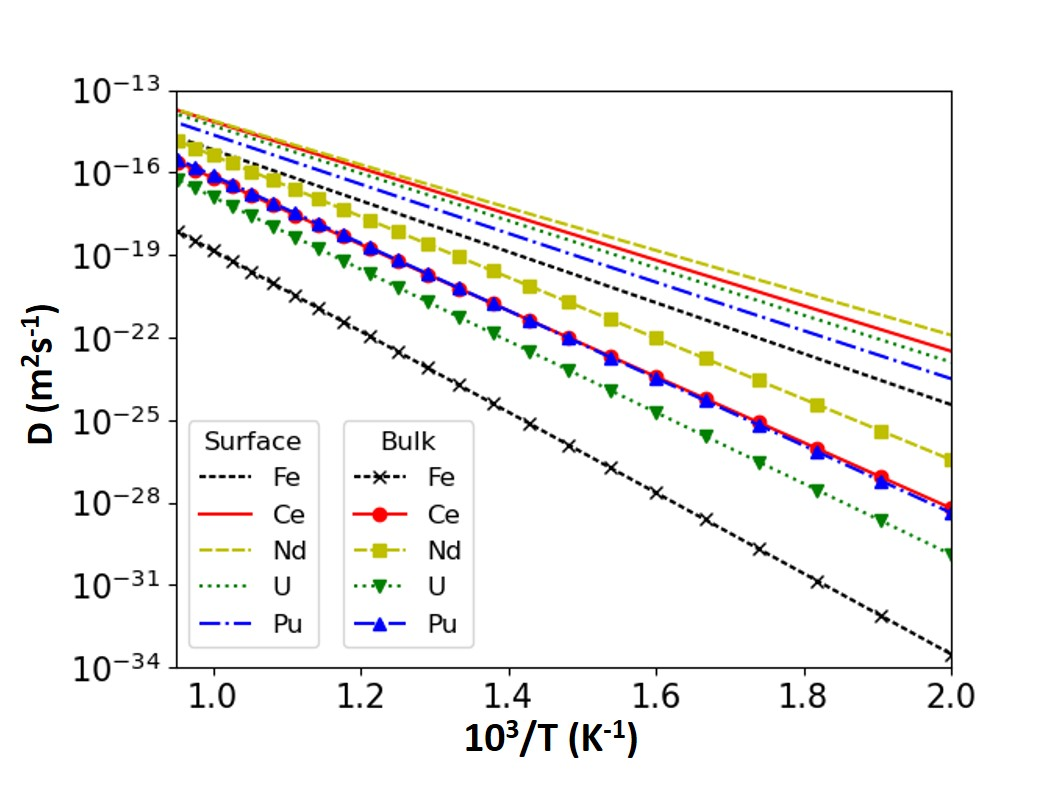
\includegraphics[width=0.8\linewidth]{surface_diff.jpg}
    \caption{The calculated self-diffusivities and solute diffusivities on the (110) surface of BCC Fe via the vacancy mechanism plotted versus inverse temperature (no markers). Bulk diffusivities (lines with markers) are shown for comparison. The corrections for magnetic disordering and electronic excitations are not applied.}
    \label{fig:diff_surface}
\end{figure}

The fitted diffusion activation energies and prefactors are listed in \Cref{tab:surface_activation_energies}. The calculated activation energies ($Q_0^F$) in \Cref{tab:surface_activation_energies} show trends similar to those of the bulk diffusivities. All solutes have lower activation energies for diffusion than Fe (self-diffusion) on the (110) surface. Nd is the fastest species, followed by Ce, with a $Q_0^F$ of 1.54 eV and 1.65 eV, respectively. One exception is that U is faster than Pu on the surface with a 0.04 eV difference in activation energy, which is opposite to what was observed in bulk Fe. Therefore, the relative trends in solute diffusion on the surface largely mirror those observed in the bulk, with surface-to-bulk diffusivity ratios remaining generally consistent for Ce, Nd, and Pu, while U exhibits a higher ratio, as shown in \Cref{fig:diff_surface}.

\begin{comment}

\begin{table}[!ht]
    \centering
    \begin{tabular}{|c|c|c|}
    \hline
     Solute & $Q_0^F$ (eV)  & $D_0$ ($\times 10^{-6} m^2s^{-1}$)  \\
     \hline
     Fe tracer  & 1.84  &1.3 \\
     Ce         & 1.65  &1.4 \\
     Nd         & 1.54  &0.4 \\
     U          & 1.70  &1.8 \\
     Pu         & 1.74  &1.3 \\
     \hline
    \end{tabular}
    \caption{Caption}
    \label{tab:surface_activation_energies}
\end{table}
    
\end{comment}

\begin{table}[!ht]
    \centering
    \caption{Activation energies and prefactors for self-diffusion and solute diffusion on the (110) surface of Fe via the vacancy mechanism.}
    \begin{tabular}{|c|c|c|c|c|c|}
    \hline
                & Fe tracer & Ce    & Nd    & U     & Pu \\
    \hline
    $Q_0^F$ (eV)& 1.84      & 1.65  &  1.54 & 1.70  & 1.74\\
    $D_0$ ($\times 10^{-6} m^2s^{-1}$)
                & 1.3       & 1.4   & 0.4   & 1.8   & 1.3\\
    \hline
    \end{tabular}
    \label{tab:surface_activation_energies}
\end{table}

\FloatBarrier
\section{Discussion}
%Lanthanide segregation to grain boundaries \cite{cao_segregation_2019}

\subsection{Bulk Diffusivities vs. Literature Data}
\label{sec:discussion1}
\noindent Our bulk diffusion results for self-diffusion show excellent agreement with experiments, as shown in \Cref{fig:self_diff}. Also, the Nd diffusivity obtained shows a very good agreement with previous calculations by Yang \textit{et al.} \cite{yang_significant_2023} using DFT and the modified nine-frequency model \cite{bocquet_migration_2017}, as shown in \Cref{fig:diff_Q}. However, the discrepancy in Ce diffusivities in \Cref{fig:diff_Q}(a) requires investigation.
In Gao \textit{et al.}'s work \cite{GAO2016316}, surprisingly, the oversized nature of solutes such as Ce, La, and Y in BCC Fe was not emphasized. They applied the standard nine-frequency model \cite{leclaire1970} using an on-lattice, relaxed solute-vacancy pair at the 1nn site without observing the two-half-vacancy configuration. Additionally, the Ce-vacancy binding energy reported by Gao \textit{et al.} (0.69 eV at 1nn) is notably lower than both our value and that of Yang \textit{et al.} \cite{yang_significant_2023}.
In contrast, Yang \textit{et al.} \cite{yang_significant_2023} explicitly observed the two-half-vacancy configurations for the Nd, Ce, and La solute-vacancy pairs in BCC Fe, similar to our findings. While we expected our results to closely match those of Yang \textit{et al.} \cite{yang_significant_2023}, the discrepancies can be attributed to differences in the migration barrier for the $\omega_{12}$ jump (a difference of 0.53 eV; see \Cref{tab:migration_barriers}) and in the 1nn Ce-vacancy binding energy (a difference of 0.28 eV; see \Cref{tab:configurations_binding}).

To investigate further, we compared the DFT parameters used in this study to those of Yang \textit{et al.} \cite{yang_significant_2023} and found them nearly identical, except for the plane-wave cutoff energy (400 eV in our case vs. 450 eV in theirs), which is unlikely to account for a 0.53 eV difference in migration barriers. We hypothesize that the discrepancy arises from the use of different pseudopotentials. A test calculation using the Ce\textunderscore3 pseudopotential (instead of the standard Ce pseudopotential used in this study) in VASP reproduced the Ce-vacancy binding energies reported by Yang \textit{et al.} \cite{yang_significant_2023}, supporting this hypothesis. For Nd, no such discrepancy was observed, likely because we used the Nd\textunderscore3 pseudopotential recommended by VASP, which is believed to be the same as that used by Yang \textit{et al.} \cite{yang_significant_2023}. The observed discrepancy and comparison highlight that the choice of the pseudopotential may affect the results. While multiple options exist for all species investigated in this study, only the pseudopotentials recommended by VASP were utilized. An exhaustive analysis of the impact of pseudopotential choice was deemed beyond the scope of this work. 



\begin{comment}

Additionally, most experimental work concerning the $\alpha$-Fe phase—relevant to the present study—has been conducted at temperatures exceeding the Curie temperature (T = 1043 K), where Fe exhibits paramagnetic behavior. Therefore, comparisons are restricted to experimental data obtained below the Curie temperature, where Fe remains in the ferromagnetic state.
\end{comment}

In \Cref{fig:diffusivities_exp}, the calculated solute and self-diffusivities are compared with experimental values for Fe, Sn, and Nb in ferromagnetic BCC Fe \cite{lubbehusen1990self, hettich1977self, torres2000diffusion, herzig2002niobium}. Sn and Nb, which are analogous to OSAs such as lanthanides and actinides, were selected for comparison due to their relatively large atomic radii compared to Fe. According to Goldschmidt atomic radii \cite{brandes2013smithells}, Fe has a radius of 1.28 Å, while Sn and Nb have radii of 1.58 Å and 1.47 Å, respectively. For the solutes of primary interest in this work, Ce and Nd exhibit radii of 1.82 Å, while no values are reported for U and Pu \cite{brandes2013smithells}.

\begin{figure}[!ht]
    \centering
    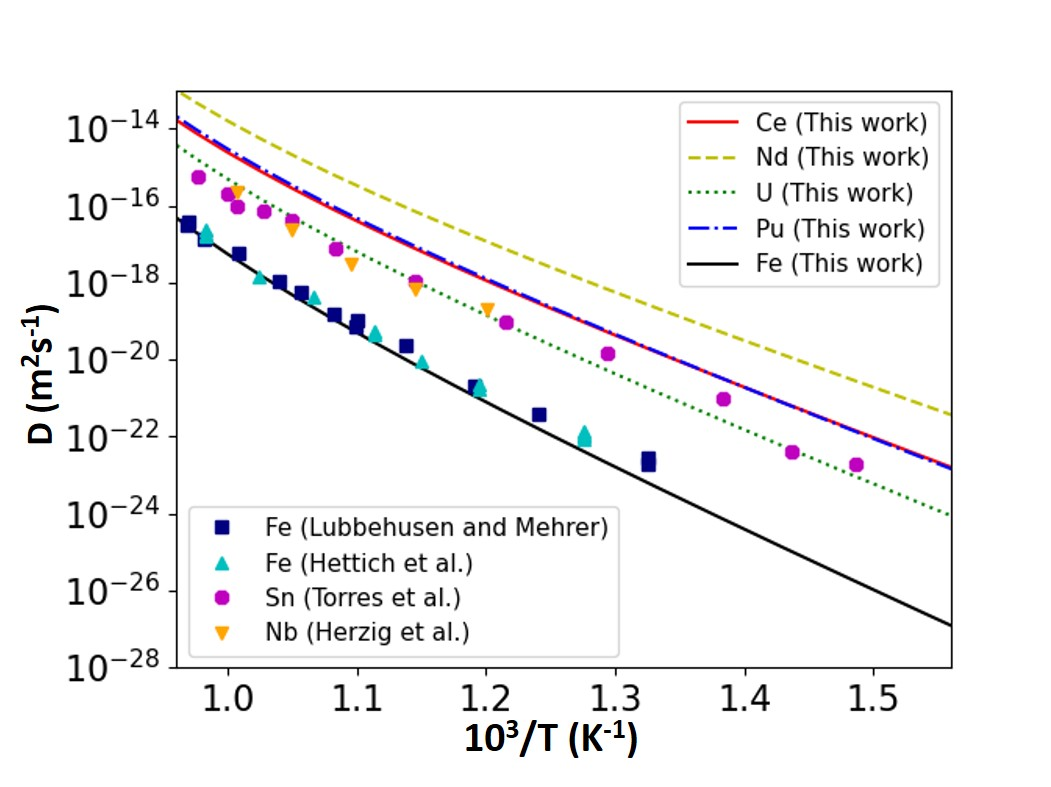
\includegraphics[width=0.8\linewidth]{experiments_fe.jpg}
    \caption{The diffusivities of Ce, Nd, U, and Pu, and self-diffusivity in bulk BCC Fe, are compared to the experimental diffusivities (scattered markers) from references \cite{lubbehusen1990self,hettich1977self,torres2000diffusion,herzig2002niobium}.}
    \label{fig:diffusivities_exp}
\end{figure}

Our results show a reasonable agreement with the experimental diffusion coefficients of Sn and Nb in BCC Fe, as shown in \Cref{fig:diffusivities_exp}. However, the activation energies are different. Sn diffusion in Fe, as reported by Torres \textit{et al.} \cite{torres2000diffusion}, has an activation energy of approximately 2.90~eV, while Nb diffusion in Fe, as reported by Herzig \textit{et al.} \cite{herzig2002niobium}, has an activation energy of approximately 2.60~eV. Both values are higher than the activation energies calculated in this work for lanthanides and actinides (See \Cref{tab:activation_energies}). This trend is consistent with the findings of Janotti \textit{et al.} \cite{janotti2004solute}, who investigated vacancy-mediated diffusion in Ni. Their study suggests that, counterintuitively, oversized solute atoms can exhibit faster diffusion (i.e., lower activation energies) via the vacancy mechanism than solutes with atomic radii more comparable to that of the host. This behavior was attributed to the characteristics expressed through the bonding of the solute d-electrons with the host Ni atoms. Extending this explanation to the present case would require an analysis of the electronic structure of solute-vacancy complexes involving f-electron solutes and d-electron host atoms, which is left for future work.

To further validate the results, comparison with experimental tracer diffusion measurements in Fe is necessary. Although numerous tracer diffusion studies have been reported in the literature \cite{neumann2011self}, lanthanide and actinide diffusion data in Fe are generally absent, except for a single study on U diffusion in $\gamma$-Fe \cite{de1967fissiographie}. Therefore, additional experimental efforts are necessary to fully validate the results presented here. 



\FloatBarrier


\subsection{Surface Diffusivities vs. Literature Data}
\label{sec:discussion2}
%Ag diffusion on Fe (110) experiment \cite{noro1996surface} adatom diffusion

\noindent To evaluate our hypothesis that vacancy-mediated surface diffusivity is comparable to GB diffusivity, we present our results in \Cref{fig:surf_diff_exp} alongside experimental data on GB diffusion from both coarse-grained \cite{inoue2007grain, bernardini1982role, hansel1985effects} and nanocrystalline Fe samples \cite{schmidt2012grain, chakravarty2009self}. Experimental surface diffusivity data in Fe are limited, but we include recent measurements at 350\textdegree C and 500\textdegree C by Taylor \textit{et al.} \cite{taylor2024directly}, which are rare direct measurements, in the same figure.

\begin{figure}[!ht]
    \centering
    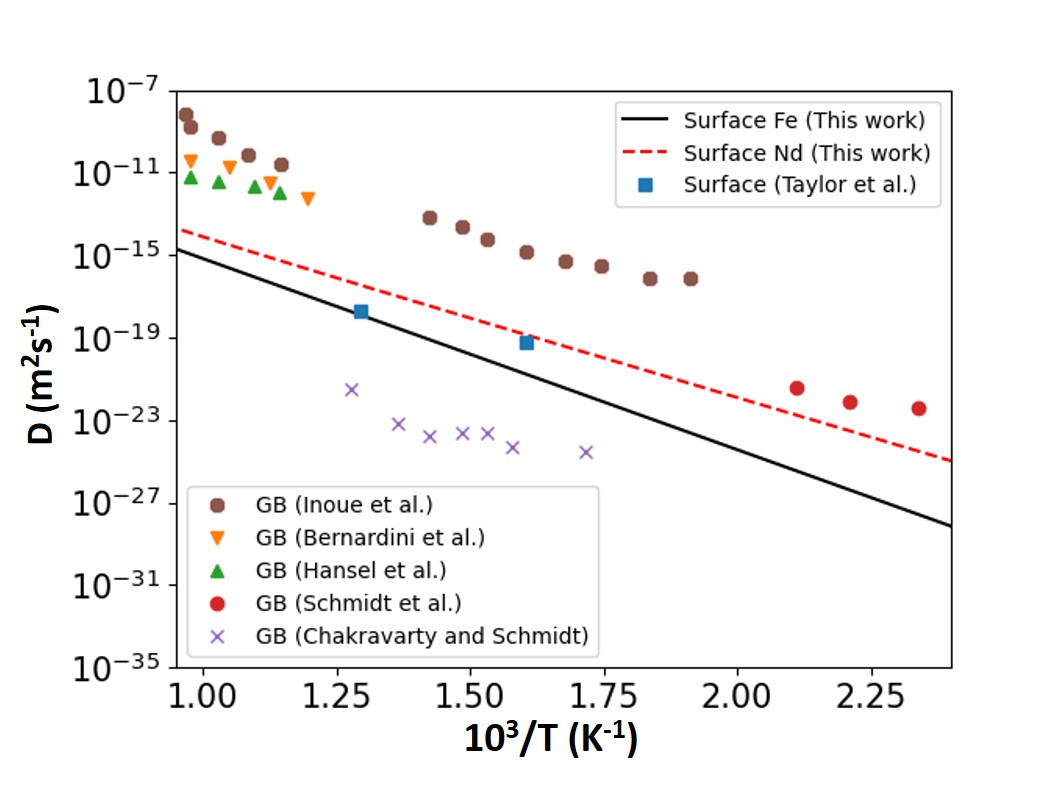
\includegraphics[width=0.8\linewidth]{surface_diff_exp.jpg}
    \caption{The calculated self-diffusivities and Nd diffusivities on the Fe (110) surface are plotted in solid black and dashed red lines, respectively. Experimental data for surface and GB self-diffusion are included for comparison \cite{taylor2024directly,inoue2007grain,bernardini1982role,hansel1985effects, schmidt2012grain, chakravarty2009self}.}
    \label{fig:surf_diff_exp}
\end{figure}

Among GB diffusion studies, Bernardini \textit{et al.} \cite{bernardini1982role} reported an activation energy of 1.72 eV for Fe self-diffusion along GBs, which aligns well with the temperature dependence observed in our results. However, their reported diffusivities are approximately four orders of magnitude higher than our calculated values. 
Inoue \textit{et al.} \cite{inoue2007grain} reported even higher GB diffusivities, along with a lower activation energy of 1.32 eV for random high-angle boundaries. 
H\"{a}nsel \textit{et al.} \cite{hansel1985effects} reported GB diffusivities that are lower than those of Bernardini \textit{et al.} \cite{bernardini1982role} and Inoue \textit{et al. }\cite{inoue2007grain} but that have an even lower activation energy of 0.94 eV.
Data from nanocrystalline samples by Schmidt \textit{et al.} \cite{schmidt2012grain} and Chakravarty \textit{et al.} \cite{chakravarty2009self} show activation energies in the range of 0.9–1.0 eV, though with smaller absolute diffusivities.
These variations highlight the strong dependence of GB diffusivity on boundary structure and orientation.
Given the wide experimental spread and the comparable activation energies observed across both GB and surface diffusion studies, it is reasonable to consider surface diffusion as a representative proxy for GB diffusion. Moreover, our surface diffusion results compare well with the only available experimental surface data, and they fall within the overall range of reported GB diffusivities, further supporting this assumption.



%Kochaev: 1.3 eV and 1.9 eV for self-interstitials and vacancies, respectively

Our results are also compared to prior theoretical studies of GB diffusion in BCC Fe using DFT \cite{kochaev_anisotropic_2023} and MD simulations \cite{starikov2020study} in \Cref{fig:surf_diff_simulations}. For clarity, only the fastest diffusion paths reported in those studies are included. While the vacancy-mediated diffusivity we calculated for the (110) surface and those reported for the $\Sigma5$(210) GB in previous works do not align with experimental measurements, other mechanisms provide better agreement. Specifically, Kochaev and L’vov \cite{kochaev_anisotropic_2023}, based on their DFT calculations, demonstrated that interstitial-mediated diffusion dominates GB self-diffusion in Fe. Similarly, MD simulations by Starikov \textit{et al.} \cite{starikov2020study} using the embedded atom method potentials also point to an interstitial mechanism as the primary diffusion mode. Their work yielded diffusivities in excellent agreement with experiments.

\begin{figure}[!ht]
    \centering
    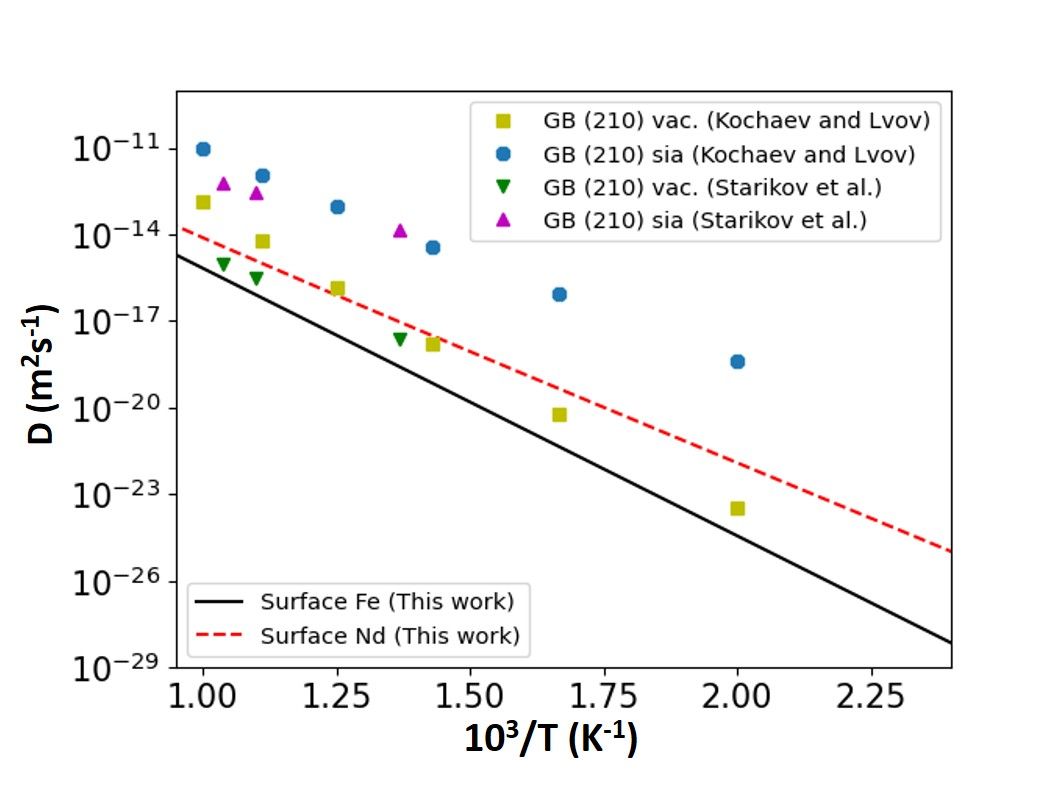
\includegraphics[width=0.8\linewidth]{surface_diff_sim.jpg}
    \caption{The calculated self-diffusivities and Nd diffusivities on the Fe (110) surface are plotted in solid black and dashed red lines, respectively. DFT results from reference \cite{kochaev_anisotropic_2023} and MD results from reference \cite{starikov2020study} are included for comparison for vacancy (vac.) and self-interstitial (sia) mechanisms.}
    \label{fig:surf_diff_simulations}
\end{figure}

These findings challenge the conventional assumption that self-diffusion along Fe GBs is vacancy-mediated \cite{balluffi1982grain, peterson1983grain, klotsman1990impurity, kwok1981}, leaving the dominant diffusion mechanism an open question. Nevertheless, in the case of the lanthanide and actinide solutes considered in this study, interstitial configurations are energetically unfavorable due to their large atomic sizes. Octahedral and dumbbell interstitial sites were tested, and interstitial formation energies for Ce and Nd were found to be at least 5 eV higher than the corresponding substitutional formation energies. Therefore, we assume that lanthanide and actinide diffusion along GBs and surfaces proceeds via a vacancy-mediated mechanism, and our reported surface diffusivities can be utilized as a good approximation for lanthanide and actinide diffusivities along Fe GBs.

%Compare to MD self-diffusion on (110) surface in references \cite{wang2010single, wang2012molecular} and on other surfaces \cite{papanicolaou2009diffusion, wen2007atomistic}

%Bernardini and co-workers employed bulk diffusivity values that were overestimated by 1-2 orders of magnitude relative to more accurate experimental data reported by Lubbehusen et al. \cite{lubbehusen1990self, hettich1977self}. These inflated bulk diffusivity values were used as input in the application of the Suzuoka analytical solution for grain boundary diffusion \cite{suzuoka1961lattice, suzuoka1964exact}.

\FloatBarrier

\section{Conclusion}
\noindent The vacancy-mediated diffusion coefficients of Ce, Nd, U, and Pu in bulk BCC Fe were calculated using DFT-derived energetics and SCMF theory. Our results indicate that lanthanides and actinides diffuse significantly faster than Fe self-diffusion in the BCC lattice, primarily due to strong vacancy drag resulting from their attractive binding to vacancies. At high temperatures ($\sim1000$~K), these solutes diffuse 2–3 orders of magnitude faster than Fe, while at lower temperatures ($\sim500$~K), the difference increases to 4–8 orders of magnitude.
The computed self-diffusivities of Fe agree well with experimental tracer diffusion data after corrections were applied to the activation energy to account for magnetic disordering and electronic excitations at elevated temperatures. Additionally, the calculated impurity diffusivities exhibit trends consistent with experimental diffusion measurements of Sn and Nb in BCC Fe, although the lanthanides and actinides are slightly faster.

The diffusivities of Ce, Nd, U, and Pu on the Fe (110) surface were calculated assuming two-dimensional vacancy-mediated diffusion. All solutes, along with vacancies, exhibited strong segregation to the first surface layer, indicating that diffusion into the bulk is unlikely under equilibrium conditions. 
Surface diffusion was found to be significantly faster than bulk diffusion, with activation energies for lanthanide and actinide diffusion reduced by 0.7–0.9~eV compared to bulk values. The calculated surface self-diffusivities show a similar temperature dependence to experimental GB diffusivities, though with lower magnitudes. This discrepancy, along with the wide scatter in reported experimental and theoretical GB diffusion data, highlights the sensitivity of GB diffusivity to boundary structure and orientation. 
While the dominant diffusion mechanism—vacancy, interstitial, or mixed—remains uncertain for GB self-diffusion, we argue that for oversized solutes such as lanthanides and actinides, vacancy-mediated diffusion is the most plausible pathway due to the high energetic cost of forming interstitial configurations. 
Therefore, we propose that the computed surface diffusivities can serve as reasonable approximations for lanthanide and actinide diffusion along GBs in Fe-based cladding materials. However, further studies on solute stability and migration along specific GB structures are needed to refine FCCI models at higher-length scales.

\section{Acknowledgments}

This work was supported by grants from the U.S. Department of Energy, Office of Nuclear Energy (DOE-NE) (DE-NE0009271, Project 22-26632). This research made use of the resources of the High-Performance Computing Center at Idaho National Laboratory, which is supported by the Office of Nuclear Energy of the U.S. Department of Energy and the Nuclear Science User Facilities under Contract No. DE-AC07-05ID14517.



\FloatBarrier
\bibliographystyle{elsarticle-num} 
\bibliography{references}
\end{document}
